\documentclass[12pt]{report}

\usepackage[a4paper,pdftex]{geometry}	% Use A4 paper margins
\usepackage[english]{babel}
\usepackage{xcolor} % Required for specifying custom colors
\usepackage{fix-cm} % Allows increasing the font size of specific fonts beyond LaTeX default specifications
\usepackage[hidelinks]{hyperref}
\usepackage{parskip}
\usepackage{color}
\usepackage{picture}
\usepackage{setspace}
\usepackage{amssymb}
\usepackage{mathtools}
\usepackage{graphicx}
\usepackage{floatrow}
\usepackage[labelformat=empty]{caption}


\usepackage{listings}
\usepackage{color}
 
\definecolor{dkgreen}{rgb}{0,0.6,0}
\definecolor{gray}{rgb}{0.5,0.5,0.5}
\definecolor{mauve}{rgb}{0.58,0,0.82}
 
\lstset{ %
  language=Octave,                % the language of the code
  basicstyle=\footnotesize,           % the size of the fonts that are used for the code
  backgroundcolor=\color{white},      % choose the background color. You must add \usepackage{color}
  showspaces=false,               % show spaces adding particular underscores
  showstringspaces=false,         % underline spaces within strings
  showtabs=false,                 % show tabs within strings adding particular underscores
  frame=single,                   % adds a frame around the code
  rulecolor=\color{black},        % if not set, the frame-color may be changed on line-breaks within not-black text (e.g. commens (green here))
  tabsize=2,                      % sets default tabsize to 2 spaces
  captionpos=b,                   % sets the caption-position to bottom
  breaklines=true,                % sets automatic line breaking
  breakatwhitespace=false,        % sets if automatic breaks should only happen at whitespace
  title=,                   % show the filename of files included with \lstinputlisting;
                                  % also try caption instead of title
  keywordstyle=\color{blue},          % keyword style
  commentstyle=\color{dkgreen},       % comment style
  stringstyle=\color{mauve},         % string literal style
  escapeinside={\%*}{*)},            % if you want to add LaTeX within your code
  morekeywords={*,...}               % if you want to add more keywords to the set
}


\setlength{\oddsidemargin}{0mm} % Adjust margins to center the colored title box
\setlength{\evensidemargin}{0mm} % Margins on even pages - only necessary if adding more content to this template

\newcommand{\HRule}[1]{\hfill \rule{0.2\linewidth}{#1}} % Horizontal rule at the bottom of the page, adjust width here

\definecolor{grey}{rgb}{0.9,0.9,0.9} % Color of the box surrounding the title - these values can be changed to give the box a different color	

\begin{document}

\thispagestyle{empty} % Remove page numbering on this page

%----------------------------------------------------------------------------------------
%	TITLE SECTION
%----------------------------------------------------------------------------------------

\colorbox{grey}{
	\parbox[t]{1.0\linewidth}{
		\centering \fontsize{50pt}{80pt}\selectfont % The first argument for fontsize is the font size of the text and the second is the line spacing - you may need to play with these for your particular title
		\vspace*{0.7cm} % Space between the start of the title and the top of the grey box
		
		\hfill Siminov Framework Version 0.9.2-Beta\\
		\hfill Developer Guide\par
		
		\vspace*{0.7cm} % Space between the end of the title and the bottom of the grey box
	}
}

%----------------------------------------------------------------------------------------

	\vfill % Space between the title box and author information

%----------------------------------------------------------------------------------------
%	AUTHOR NAME AND INFORMATION SECTION
%----------------------------------------------------------------------------------------

	{\centering \large 
\hfill Siminov Framework \\
\hfill \texttt{http://www.siminov.github.com/android-orm} \\

\HRule{1pt}} % Horizontal line, thickness changed here

%----------------------------------------------------------------------------------------

\clearpage % Whitespace to the end of the page


\noindent
%%%%%%%%%%%%%%%%%%%%%%%%%%%%%%%%%%%%%%%%%%%%%%%%%%%%%%%%%%%%%%%%%%%%%%%%%%%%%%%%%%%%%%%%%%%%%%%%%%%%%%%%%%%%%%%%%%%%%%%%
%set the number of sectioning levels that get number and appear in the contents
\pagenumbering{gobble}
\setcounter{secnumdepth}{3}
\setcounter{tocdepth}{3}


\tableofcontents

%%%%%%%%%%%%%%%%%%%%%%%%%%%%%%%%%%%%%%%%%%%%%%%%%%%%%%%%%%%%%%%%%%%%%%%%%%%%%%%%%%%%%%%%%%%%%%%%%%%%%%%%%%%%%%%%%%%%%%%%

%%%%%%%%%%%%%%%%%%%%%%%%%%%%%%%%%%%%%%%%%%%%%%%%%%%%%%%%%%%%%%%%%%%%%%%%%%%%%%%%%%%%%%%%%%%%%%%%%%%%%%%%%%%%%%%%%%%%%%%%
\newpage
\addcontentsline{toc}{chapter}{Preface}
\begin{flushleft}
	\textbf{\emph{\Large{Preface}}}
\end{flushleft}

\small
Working with both Object-Oriented software and Relational Databases can be cumbersome and time consuming. Development costs are significantly higher due to a paradigm mismatch between how data is represented in objects versus relational databases. Siminov is an Object/Relational Mapping solution for Android environments. The term Object/Relational Mapping refers to the technique of mapping data from an object model representation to a relational data model representation (and visa versa). See \url{http://en.wikipedia.org/wiki/Object-relational_mapping} for a good high-level discussion.


\begin{center}
	\colorbox{grey}{
		\parbox[t]{.8\linewidth}{
			\fontsize{11pt}{11pt}\selectfont % The first argument for fontsize is the font size of the text and the second is the line spacing - you may need to play with these for your particular title
			\vspace*{0.7cm} % Space between the start of the title and the top of the grey box
		
			\hfill \textbf{Note} \\
			\hfill While having a strong background in SQL is not required to use Android-Siminov, having a basic understanding of the concepts can greatly help you understand Siminov more fully and quickly. Probably the single best background is an understanding of data modeling principles. You might want to consider these resources as a good starting point: \url{http://en.wikipedia.org/wiki/Data_modeling}\\
		
			\vspace*{0.7cm} % Space between the end of the title and the bottom of the grey box
		}
}

\end{center}


Siminov not only takes care of the mapping from Java classes to database tables (and from Java data types to SQL data types), but also provides data query and retrieval facilities. It can significantly reduce development time otherwise spent with manual data handling in SQLite. Siminov design goal is to relieve the developer from 99% of common data persistence-related programming tasks by eliminating the need for manual, hand-crafted data processing using SQLite. However, unlike many other persistence solutions, Siminov does not hide the power of SQLite from you and guarantees that your investment in relational technology and knowledge is as valid as always.

Siminov may not be the best solution for data-centric applications that only use stored-procedures to implement the business logic in the database, it is most useful with object-oriented domain models and business logic in the Java-based. However, Siminov can certainly help you to remove or encapsulate vendor-specific SQLite code and will help with the common task of result set translation from a tabular representation to a graph of objects.


\section{Get Involved}

Use Siminov and report any bugs or issues you find. See \url{https://github.com/Siminov/android-orm/issues} for details. Try your hand at fixing some bugs or implementing enhancements. Again, see \url{https://github.com/Siminov/android-orm/issues}. Engage with the community using mailing lists, forums, IRC, or other ways listed at \url{https://github.com/Siminovl}. Help improve or translate this documentation. Contact us on the developer mailing list if you have interest.Spread the word. Let the rest of your organization know about the benefits of Siminov.


\section{Getting Started Guide}

New users may want to first look through the Siminov Getting Started Guide for basic information as well as tutorials. Even seasoned veterans may want to considering perusing the sections pertaining to build artifacts for any changes.

%%%%%%%%%%%%%%%%%%%%%%%%%%%%%%%%%%%%%%%%%%%%%%%%%%%%%%%%%%%%%%%%%%%%%%%%%%%%%%%%%%%%%%%%%%%%%%%%%%%%%%%%%%%%%%%%%%%%%%%%
\newpage
\chapter {\Large{Overview}}

Siminov ORM component is a native object relationship mapping framework, which handles all activities related to database.


\begin{figure}[!htbp]
	\centering
		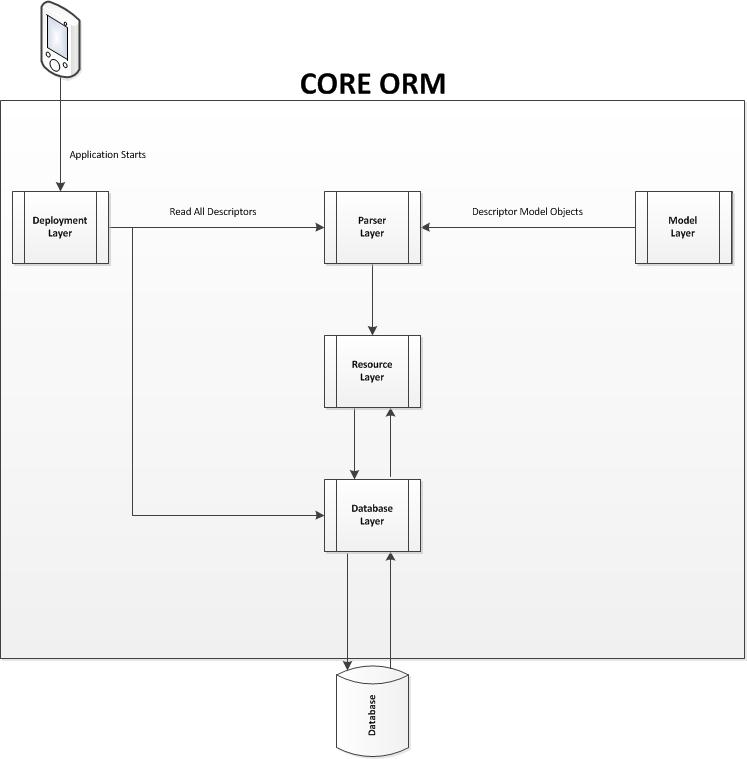
\includegraphics[height=11.5cm]{Resources/siminov_architecture.jpg}
	\caption{Siminov ORM Layers}
\end{figure}


\section{Features}
\begin{enumerate}

	\small \item Handles application deployment.
	\small \item Provides simple and clean orm for every platform.
	\small \item Easy to configure and develop using xml or annotations.
	\small \item Provides encryption implementations.

\end{enumerate}
%%%%%%%%%%%%%%%%%%%%%%%%%%%%%%%%%%%%%%%%%%%%%%%%%%%%%%%%%%%%%%%%%%%%%%%%%%%%%%%%%%%%%%%%%%%%%%%%%%%%%%%%%%%%%%%%%%%%%%%%
\newpage
\chapter {\Large{Configuration}}

\begin{figure}[htbp]
	\centering
		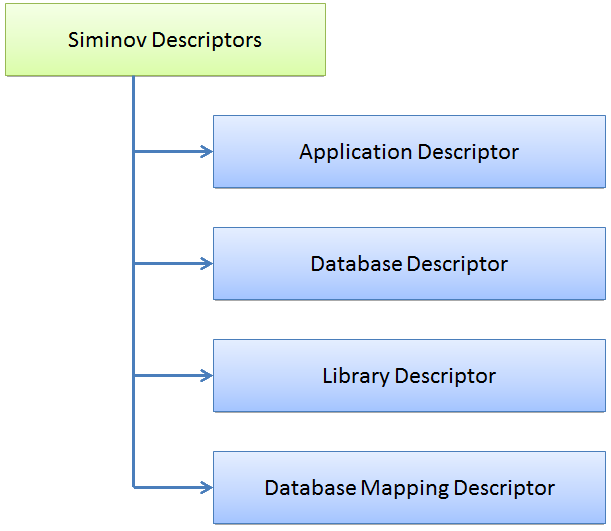
\includegraphics[height=8cm]{Resources/siminov_descriptors.png}
\end{figure}

\par
Siminov Framework works based on a set of defined descriptors which can be broadly classified as \textbf{ApplicationDescriptor.si.xml}, \textbf{DatabaseDescriptor.si.xml}, \textbf{LibraryDescriptor.si.xml}, \textbf{DatabaseMappingDescriptor.si.xml}.

\par
All these descriptor should will be placed in application assests folder. 

\newpage
\begin{figure}[!htbp]
	\centering
		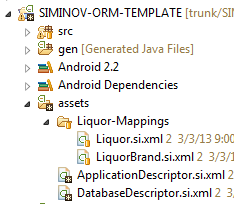
\includegraphics[height=8cm]{Resources/application_assests_structure.png}
\end{figure}


\begin{center}
	\colorbox{grey}{
		\parbox[t]{.8\linewidth}{
			\fontsize{11pt}{11pt}\selectfont % The first argument for fontsize is the font size of the text and the second is the line spacing - you may need to play with these for your particular title
			\vspace*{0.1cm} % Space between the start of the title and the top of the grey box
		
			\hfill \textbf{Note} \\

			\hfill 	
			\begin{enumerate}
			
				\item \small All descriptor file name should end with \textbf{.si.xml}.

			\end{enumerate}

			\vspace*{0.0cm} % Space between the end of the title and the bottom of the grey box
		}
	}

\end{center}



\newpage
\section{Application Descriptor (ApplicationDescriptor.si.xml) Configuration} 
	Application Descriptor is the one who connects application to Siminov framework. It provide basic information about application, which defines the behaviour of application.

\lstinputlisting[language=XML]{Resources/application_descriptor.txt}

\newpage
\textbf{Example}: ApplicationDescriptor.si.xml File Of Siminov Template Application.
\lstinputlisting[language=XML]{Resources/siminov_template_application_descriptor.txt}

			\begin{center}
				\colorbox{grey}{
					\parbox[t]{.8\linewidth}{
						\fontsize{11pt}{11pt}\selectfont % The first argument for fontsize is the font size of the text and the second is the line spacing - you may need to play with these for your particular title
						\vspace*{0.1cm} % Space between the start of the title and the top of the grey box
		
						\hfill \textbf{Note} \\

			
						Application Developer can provide their own properties also, and by using following API's they can use properties.

						\hfill 	
						\begin{enumerate}
							\item \small Get Properties - getProperties(): It will return all properties associated with Application Descriptor.
							\item \small Get Property - getProperty(Name of Property): It will return property value associated with property name provided.
							\item \small Contains Property - containsProperty(Name of Property): It will return TRUE/FALSE whether property exists or not.
							\item \small Add Property - addProperty(Name of Property, Value of Property ): It will add new property to the  collection of Application Descriptor properties.
							\item \small Remove Property - removeProperty(Name of Property): It will remove property from Application Descriptor properties based on name provided.
						\end{enumerate}

						\vspace*{0.0cm} % Space between the end of the title and the bottom of the grey box
				}
			}

		\end{center}


\textbf{Application Descriptor Elements}: 

\begin{enumerate}
	
	\item \small General Properties About Application.
	
		\begin{enumerate}

			\item \small \textbf{name*} : Name of application. It is mandatory field. If any resources is created by Siminov then it will be under this folder name.

			\begin{figure}[htbp]
				\centering
					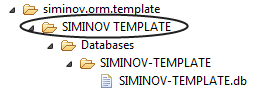
\includegraphics[height=3cm]{Resources/siminov_template_application_data_folder_structure_for_application_name.png}
			\end{figure}


			\item \small \textbf{description}: Description of application. It is optional field.
			\item \small \textbf{version}: Version of application. It is mandatory field. Default is 0.0.

		\end{enumerate}

	\item \small Framework Performance Properties.
		
		\begin{enumerate}

			\item \small \textbf{load\_initially}: \textit{TRUE}/\textit{FALSE}: ORM(Object Relational Mapping) to be done at start of application or at the time when its needed. It is optional field. By default its false, means mapping is done when its required. 

			\begin{center}
				\colorbox{grey}{
					\parbox[t]{.8\linewidth}{
						\fontsize{11pt}{11pt}\selectfont % The first argument for fontsize is the font size of the text and the second is the line spacing - you may need to play with these for your particular title
						\vspace*{0.1cm} % Space between the start of the title and the top of the grey box
		
						\hfill \textbf{Note} \\

						\hfill 	
						\begin{enumerate}
			
							\item \small If load\_initially is false then application will start quickly.

						\end{enumerate}

						\vspace*{0.0cm} % Space between the end of the title and the bottom of the grey box
				}
			}

		\end{center}

		
		\end{enumerate}

	\item \small Path Of Database Descriptor's Used In Application.

		\begin{itemize}

			\item \small Path of all database descriptor's used in application.
			\item \small Every database descriptor will have its own database object.
		
		\end{itemize}

	\item \small Event Handlers Implemented By Application 

		\begin{itemize}

			\item \small Siminov Framework provides two type of event handlers
			
				\begin{itemize}
					\item \small \textbf{ISiminovEvents}: It contains events associated with life cycle of Siminov Framework. such as \textbf{siminovInitialized}, \textbf{firstTimeSiminovInitialized}, \textbf{siminovStopped}.
					\item \small \textbf{IDatabaseEvents}: It contains events associated with database operations. such as \textbf{databaseCreated}, \textbf{databaseDropped}, \textbf{tableCreated}, \textbf{tableDropped}, \textbf{indexCreated}, 													\textbf{indexDropped}.
		
				\end{itemize}

			\item \small Application can implement these event handlers based on there requirement.

		\end{itemize}

\end{enumerate}

\begin{center}
	\colorbox{grey}{
		\parbox[t]{.8\linewidth}{
			\fontsize{11pt}{11pt}\selectfont % The first argument for fontsize is the font size of the text and the second is the line spacing - you may need to play with these for your particular title
			\vspace*{0.1cm} % Space between the start of the title and the top of the grey box
		
			\hfill \textbf{Note} \\

			\hfill 	
			\begin{enumerate}
			
				\item \small Application descriptor file name should always be same as ApplicationDescriptor.si.xml only.

				\item \small It should always be in root folder of application assests.

			\end{enumerate}

			\vspace*{0.0cm} % Space between the end of the title and the bottom of the grey box
		}
}

\end{center}

	\par
		\textbf{Example:} Siminov Template Application.
		\begin{figure}[htbp]
			\centering
				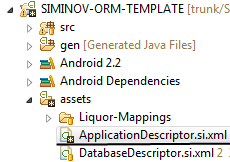
\includegraphics[height=4.5cm]{Resources/siminov_application_template_application_descriptor_path_example.png}
		\end{figure}


\newpage
\section{Database Descriptor (DatabaseDescriptor.si.xml) Configuration}
	Database Descriptor is the one who defines the schema of database.
	
\lstinputlisting[language=XML]{Resources/database_descriptor.txt}

\newpage
\textbf{Example}: DatabaseDescriptor.si.xml File Of Siminov Template Application.
\lstinputlisting[language=XML]{Resources/siminov_template_database_descriptor.txt}


			\begin{center}
				\colorbox{grey}{
					\parbox[t]{.8\linewidth}{
						\fontsize{11pt}{11pt}\selectfont % The first argument for fontsize is the font size of the text and the second is the line spacing - you may need to play with these for your particular title
						\vspace*{0.1cm} % Space between the start of the title and the top of the grey box
		
						\hfill \textbf{Note} \\

			
						Application Developer can provide their own properties also, and by using following API's they can use properties.

						\hfill 	
						\begin{enumerate}
							\item \small Get Properties - getProperties(): It will return all properties associated with Database Descriptor.
							\item \small Get Property - getProperty(Name of Property): It will return property value associated with property name provided.
							\item \small Contains Property - containsProperty(Name of Property): It will return TRUE/FALSE whether property exists or not.
							\item \small Add Property - addProperty(Name of Property, Value of Property ): It will add new property to the  collection of Database Descriptor properties.
							\item \small Remove Property - removeProperty(Name of Property): It will remove property from Database Descriptor properties based on name provided.
						\end{enumerate}

						\vspace*{0.0cm} % Space between the end of the title and the bottom of the grey box
				}
			}

		\end{center}


\textbf{Database Descriptor Elements}: 

\begin{enumerate}

	\item \small General Properties About Database.

		\begin{enumerate}

			\item \small \textbf{database\_name*}: Name of database. It is mandatory field. All database files (.db)'s will be placed under the this folder name.

			\begin{figure}[htbp]
				\centering
					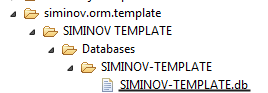
\includegraphics[height=3cm]{Resources/siminov_template_application_data_folder_structure_for_database_name.png}
			\end{figure}

			\item \small \textbf{type}: It defines the type of database. It is optional field. Default is sqlite.

			\item \small \textbf{description}: Description of database. It is optional field.
			\item \small \textbf{is\_locking\_required}: \textbf{TRUE}/\textbf{FALSE}, Control whether or not the database is made thread-safe by using locks around critical sections. 
				
				\par
				This is pretty expensive, so if you know that your DB will only be used by a multi threads then you should set this to true. 

				\par
				The default is false. It is optional field. 
			
			\begin{center}
				\colorbox{grey}{
					\parbox[t]{.8\linewidth}{
						\fontsize{11pt}{11pt}\selectfont % The first argument for fontsize is the font size of the text and the second is the line spacing - you may need to play with these for your particular title
						\vspace*{0.1cm} % Space between the start of the title and the top of the grey box
		
						\hfill \textbf{Note} \\

						\hfill 	Siminov does not provide any security for database. If you want your database data needs to encrypted, then you can include SQLCipher implementation provided by Siminov framework in your application. For more detail see SQLCipher Encryption section of this developer guide.

						\vspace*{0.0cm} % Space between the end of the title and the bottom of the grey box
					}
			}

			\end{center}

			\item \small \textbf{external\_storage}:It specifies whether database resources needs to be saved on external storage or not (SDCard). It is optinal field. Default is false.

		\end{enumerate}


	\item \small Paths Of Database Mapping Descriptor Needed Under This Database Descriptor. 

			\begin{center}
				\colorbox{grey}{
					\parbox[t]{.8\linewidth}{
						\fontsize{11pt}{11pt}\selectfont % The first argument for fontsize is the font size of the text and the second is the line spacing - you may need to play with these for your particular title
						\vspace*{0.1cm} % Space between the start of the title and the top of the grey box
		
						\hfill \textbf{Note} \\

						\hfill 

						\begin{enumerate}

							\item \small Provide full database mapping descriptor file path if you have used xml format to define ORM.

							\item \small Provide full class path of database mapping descriptor POJO class if you have used annotation to define ORM.
	
						\end{enumerate}

						\vspace*{0.0cm} % Space between the end of the title and the bottom of the grey box
					}
			}

			\end{center}

	\item \small Paths Of Library Descriptor Needed Under This Database Descriptor.

			\begin{center}
				\colorbox{grey}{
					\parbox[t]{.8\linewidth}{
						\fontsize{11pt}{11pt}\selectfont % The first argument for fontsize is the font size of the text and the second is the line spacing - you may need to play with these for your particular title
						\vspace*{0.1cm} % Space between the start of the title and the top of the grey box
		
						\hfill \textbf{Note} \\

						\hfill 

						\begin{enumerate}

							\item \small Provide full package name under which LibraryDescriptor.si.xml file is placed.

							\item \small Siminov framework will automatically read LibraryDescriptor.si.xml file defined under package name provided.
	
						\end{enumerate}

						\vspace*{0.0cm} % Space between the end of the title and the bottom of the grey box
					}
			}

			\end{center}

\end{enumerate}


	\begin{center}
		\colorbox{grey}{
			\parbox[t]{.8\linewidth}{
				\fontsize{11pt}{11pt}\selectfont % The first argument for fontsize is the font size of the text and the second is the line spacing - you may need to play with these for your particular title
				\vspace*{0.1cm} % Space between the start of the title and the top of the grey box
		
				\hfill \textbf{Note} \\

				\hfill 

				\begin{enumerate}

					\item \small You can specify any name for DatabaseDescriptor.si.xml file.

					\item \small If any database folder is created, it will be on the name of database defined in DatabaseDescriptor.si.xml file.
	
				\end{enumerate}

				\vspace*{0.0cm} % Space between the end of the title and the bottom of the grey box
			}
	}

\end{center}

\newpage
	\par
		\textbf{Example:} DatabaseDescriptor.si.xml file path
		\begin{figure}[htbp]
			\centering
				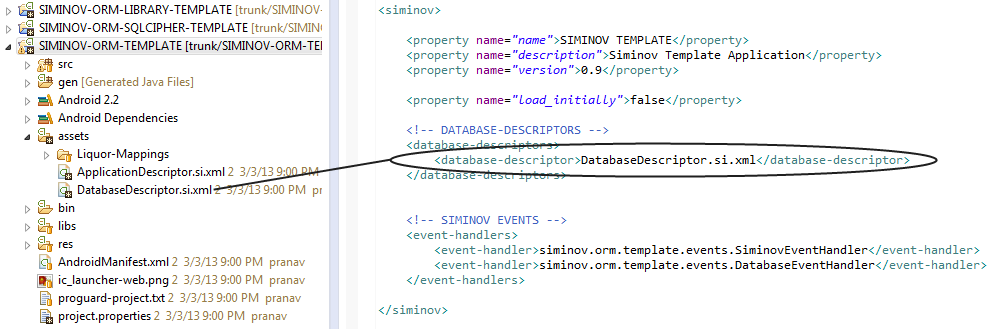
\includegraphics[height=6cm]{Resources/siminov_template_application_database_descriptor_path_example.png}
		\end{figure}




\newpage
\section{Library Descriptor (LibraryDescriptor.si.xml) Configuration}
	Library Descriptor is the one who defines the properties of library.

\lstinputlisting[language=XML]{Resources/library_descriptor.txt}

\textbf{Example}: LibraryDescriptor.si.xml File Of Siminov Library Template.
\lstinputlisting[language=XML]{Resources/siminov_library_template_library_descriptor.txt}

			\begin{center}
				\colorbox{grey}{
					\parbox[t]{.8\linewidth}{
						\fontsize{11pt}{11pt}\selectfont % The first argument for fontsize is the font size of the text and the second is the line spacing - you may need to play with these for your particular title
						\vspace*{0.1cm} % Space between the start of the title and the top of the grey box
		
						\hfill \textbf{Note} \\

			
						Application Developer can provide their own properties also, and by using following API's they can use properties.

						\hfill 	
						\begin{enumerate}
							\item \small Get Properties - getProperties(): It will return all properties associated with Library Descriptor.
							\item \small Get Property - getProperty(Name of Property): It will return property value associated with property name provided.
							\item \small Contains Property - containsProperty(Name of Property): It will return TRUE/FALSE whether property exists or not.
							\item \small Add Property - addProperty(Name of Property, Value of Property ): It will add new property to the  collection of Library Descriptor properties.
							\item \small Remove Property - removeProperty(Name of Property): It will remove property from Library Descriptor properties based on name provided.
						\end{enumerate}

						\vspace*{0.0cm} % Space between the end of the title and the bottom of the grey box
				}
			}

		\end{center}


\newpage
\textbf{Library Descriptor Elements}: 

\begin{enumerate}

	\item \small General Properties Of Library.
		
		\begin{enumerate}

			\item \small \textbf{name*}: Name of library. It is mandatory field.
			\item \small \textbf{description}: Description of library. It is optional field.
		
		\end{enumerate}

	\item \small Database Mapping Paths Needed Under This Database Descriptor.	

			\begin{center}
				\colorbox{grey}{
					\parbox[t]{.8\linewidth}{
						\fontsize{11pt}{11pt}\selectfont % The first argument for fontsize is the font size of the text and the second is the line spacing - you may need to play with these for your particular title
						\vspace*{0.1cm} % Space between the start of the title and the top of the grey box
		
						\hfill \textbf{Note} \\

						\hfill 

						\begin{enumerate}

							\item \small Provide full database mapping descriptor file path if you have used xml format to define ORM.

							\item \small Provide full class path of database mapping descriptor POJO class if you have used annotation to define ORM.
	
						\end{enumerate}

						\vspace*{0.0cm} % Space between the end of the title and the bottom of the grey box
					}
			}

			\end{center}

\end{enumerate}

	\begin{center}
		\colorbox{grey}{
			\parbox[t]{.8\linewidth}{
				\fontsize{11pt}{11pt}\selectfont % The first argument for fontsize is the font size of the text and the second is the line spacing - you may need to play with these for your particular title
				\vspace*{0.1cm} % Space between the start of the title and the top of the grey box
		
				\hfill \textbf{Note} \\

				\hfill 

				\begin{enumerate}

					\item \small Library descriptor file name should be same as LibraryDescriptor.si.xml.

					\item \small It should always be in root package specified in DatabaseDescriptor.si.xml file.
	
				\end{enumerate}

				\vspace*{0.0cm} % Space between the end of the title and the bottom of the grey box
			}
		}

\end{center}

		\par
		\textbf{Example:} LibraryDescriptor.si.xml file path
		\begin{figure}[htbp]
			\centering
				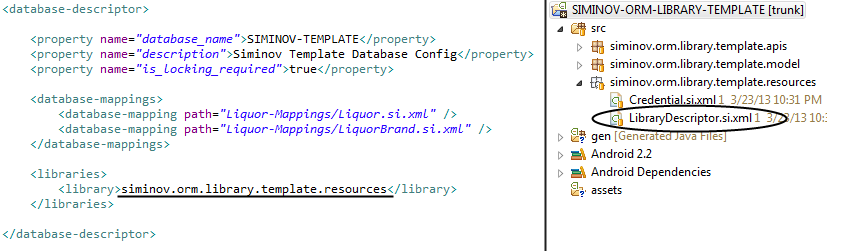
\includegraphics[height=6.2cm]{Resources/siminov_library_template_path_example.png}
		\end{figure}



\newpage
\section{Database Mapping Descriptor (DatabaseMappingDescriptor.si.xml) Configuration}
	
Database Mapping Descriptor is one which does ORM, it maps POJO class to database table.
\lstinputlisting[language=XML]{Resources/database_mapping_descriptor.txt}


\textbf{Example}: DatabaseMappingDescriptor.si.xml File Of Siminov Library Template.
\lstinputlisting[language=XML]{Resources/siminov_template_application_liquor_database_mapping_descriptor.txt}


\newpage
\textbf{Database Mapping Descriptor Elements}:

\begin{enumerate}

	\item \small \textbf{TABLE TAG}: It map database table to its corresponding POJO class.

		\begin{enumerate}

			\item \small \textbf{table\_name*}: Name of table. It is mandatory field.
			\item \small \textbf{class\_name*}: Name of POJO class name which is to be mapped to table name. It is mandatory field.

		\end{enumerate}


	\item \small \textbf{COLUMN TAG}: It map database table column to its corresponding variable of POJO class.

		\begin{enumerate}

			\item \small \textbf{column\_name*}: Name of column. It is mandatory field.
			\item \small \textbf{variable\_name*}: Name of variable. It is mandatory field.

		\end{enumerate}

		
		\par
		\textbf{Properties Of Column Tag}
	
		\begin{enumerate}

			\item \small \textbf{type*}: Java variable type (\textit{int}, \textit{java.lang.Integer}, \textit{long}, \textit{java.lang.Long}, \textit{float}, \textit{java.lang.Float}, \textit{boolean}, \textit{java.lang.Boolean}, \textit{char}, \textit{java.lang.Character}, \textit{java.lang.String}, \textit{byte}, \textit{java.lang.Byte}, \textit{void}, \textit{java.lang.Void}, \textit{short}, \textit{java.lang.Short}). It is mandatory property. 
				\par
				For more details see Data Type section of this developer guide.
			
			\item \small \textbf{primary\_key}: \textit{TRUE}/\textit{FALSE}. It defines wheather the column is primary key of table or not. It is optional property. Default value is false.
			\item \small \textbf{not\_null}: \textit{TRUE}/\textit{FALSE}. It defines wheather the column value can be empty or not. It is optional property. Default value is false.
			\item \small \textbf{unique}: \textit{TRUE}/\textit{FALSE}. It defines wheather the column value should be unique or not. It is optional property. Default value is false.
			\item \small \textbf{default}: It define the default value of column. It is optional property.
			\item \small \textbf{check}: It is used to put condition on column value. It is optional property.

		\end{enumerate}

			\begin{center}
				\colorbox{grey}{
					\parbox[t]{.8\linewidth}{
						\fontsize{11pt}{11pt}\selectfont % The first argument for fontsize is the font size of the text and the second is the line spacing - you may need to play with these for your particular title
						\vspace*{0.1cm} % Space between the start of the title and the top of the grey box
		
						\hfill \textbf{Note} \\

			
						Application Developer can provide their own properties also, and by using following API's they can use properties.

						\hfill 	
						\begin{enumerate}
							\item \small Get Properties - getProperties(): It will return all properties associated with Database Mapping Descriptor Column.
							\item \small Get Property - getProperty(Name of Property): It will return property value associated with property name provided.
							\item \small Contains Property - containsProperty(Name of Property): It will return TRUE/FALSE whether property exists or not.
							\item \small Add Property - addProperty(Name of Property, Value of Property ): It will add new property to the  collection of Database Mapping Descriptor Column properties.
							\item \small Remove Property - removeProperty(Name of Property): It will remove property from Database Mapping Descriptor Column properties based on name provided.
						\end{enumerate}

						\vspace*{0.0cm} % Space between the end of the title and the bottom of the grey box
				}
			}

		\end{center}


	\item \small \textbf{INDEX TAG}: It defines the stucture of  index needed on the table.

		\begin{enumerate}

			\item \small \textbf{name*}: Name of the index. It is mandatory field.
			\item \small \textbf{unique}: \textit{TRUE}/\textit{FALSE}. It defines wheather index needs to be unique or not. It is not mandatory property. Default value is false.
				
				\par
				(A unique index guarantees that the index key contains no duplicate values and therefore every row in the table is in some way unique). 

		\end{enumerate}


		\par
		\textbf{Index Column Tag}

		\begin{enumerate}

			\item \small \textbf{column}: Name of columns included in index. Atleast one column should be included.

		\end{enumerate}
		

	
	\item \small \textbf{RELATIONSHIPS TAG}: It defines relationship between object.

		\par
		Relationship can be of four types:

		\begin{enumerate}

			\item \small \textbf{ONE-TO-ONE}: \textit{\[<one-to-one>\]} In a one-to-one relationship, each row in one database table is linked to 1 and only 1 other row in another table.

			\item \small \textbf{ONE-TO-MANY}: \textit{\[<one-to-many>\]} In a one-to-many relationship, each row in the related to table can be related to many rows in the relating table. This effectively save storage as the related record does not need to be stored multiple times in the relating table.

			\item \small \textbf{MANY-TO-ONE}: \textit{\[<many-to-one>\]} In a many-to-one relationship one entity (typically a column or set of columns) contains values that refer to another entity (a column or set of columns) that has unique values.
	
			\item \small \textbf{MANY-TO-MANY}: \textit{\[<many-to-many>\]} In a many-to-many relationship, one or more rows in a table can be related to 0, 1 or many rows in another table. A mapping table is required in order to implement such a relationship.
	
		\end{enumerate}

			
		\textbf{Relationship Attributes}

		\begin{enumerate}

			\item \small \textbf{refer*}: Name of variable which needs to be mapped. It is mandatory field.

			\item \small \textbf{refer\_to*}: Class name of mapped variable. It is mandatory field.

			\item \small \textbf{on\_update}: \textit{cascade}/\textit{restrict}/\textit{no\_action}/\textit{set\_null}/\textit{set\_default}. It defines action needs to be done, when update occur.

			\item \small \textbf{on\_delete}: \textit{cascade}/\textit{restrict}/\textit{no\_action}/\textit{set\_null}/\textit{set\_default}. It defines action needs to be done, when delete occur.
		
		\end{enumerate}

		\textbf{Relationship Properties}

		\begin{enumerate}

			\item \small \textbf{load}: It defines whether it need to be load or not.
			
		\end{enumerate}
		
\end{enumerate}

\newpage
\begin{center}
		\colorbox{grey}{
			\parbox[t]{.8\linewidth}{
				\fontsize{11pt}{11pt}\selectfont % The first argument for fontsize is the font size of the text and the second is the line spacing - you may need to play with these for your particular title
				\vspace*{0.1cm} % Space between the start of the title and the top of the grey box
		
				\hfill \textbf{Note} \\

				\hfill 

				\begin{enumerate}

					\item \small Application developer can assign any name to DatabaseMappingDescriptor.si.xml file.

					\item \small It descriptor file should be in same place as per defined in DatabaseDescriptor.si.xml file.
	
				\end{enumerate}

				\vspace*{0.0cm} % Space between the end of the title and the bottom of the grey box
			}
		}

\end{center}

		\par
		\textbf{Example:} DatabaseMappingDescriptor.si.xml file path
		\begin{figure}[htbp]
			\centering
				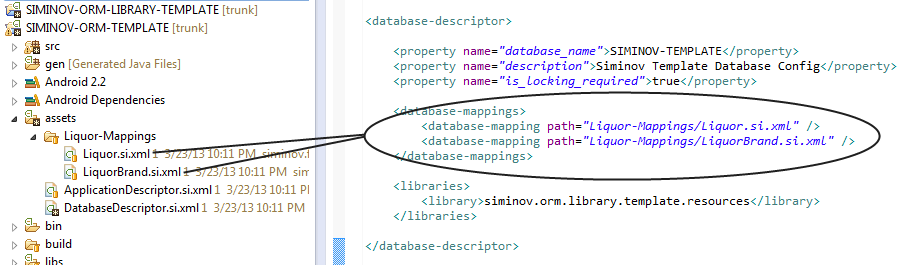
\includegraphics[height=6cm]{Resources/siminov_template_database_descriptor_mapping_path_example.png}
		\end{figure}


\newpage
\section{Database Mapping Descriptor Through Annotation}
Annotation is another way to do ORM, it maps POJO class to database table.

\par
(Annotations provide data about a program that is not part of the program itself. They have no direct effect on the operation of the code they annotate)

\lstinputlisting[language=Java]{Resources/database_mapping_descriptor_annotation.txt}

\textbf{Example}: Liquor Class Of Siminov Template Application.
\lstinputlisting[language=XML]{Resources/siminov_template_application_liquor_annotation_class.txt}

\newpage
\textbf{Different Annotation Tags}:

\begin{enumerate}

	\item \small \textbf{@Table}: It map database table to its corresponding POJO class.
		
		\begin{enumerate}

			\item \small \textbf{tableName*}: Name of table. It is mandatory field.

		\end{enumerate}
	

	\item \small \textbf{@Indexes}: It contain all index required on table.


	\item \small \textbf{@Index}: It defines the stucture of  index needed on the table.

		\begin{enumerate}

			\item \small \textbf{name*}: Name of the index. It is mandatory field.
			\item \small \textbf{unique}: \textit{TRUE}/\textit{FALSE}. It defines wheather index needs to be unique or not. It is not mandatory property. Default value is false.
				
				\par
				(A unique index guarantees that the index key contains no duplicate values and therefore every row in the table is in some way unique). 


		\end{enumerate}

		
		\par
		\textbf{Index Column Tag}

		\begin{enumerate}

			\item \small \textbf{column}: Name of columns included in index. Atleast one column should be included.

		\end{enumerate}

	\item \small \textbf{@Column}: It map database table column to its corresponding variable of POJO class.

		\begin{enumerate}

			\item \small \textbf{columnName*}: Name of column. It is mandatory field.

		\end{enumerate}

		\par
		\textbf{Properties Of Column: @Properties}: It contain all properties needed by column.
	
		\par
		\textbf{Properties Of Column Tag: @Property}: This tag defines a perticular property of column.

		\begin{enumerate}

			\item \small \textbf{primary\_key} | \textbf{ColumnProperty}.\textbf{PRIMARY\_KEY}: \textit{TRUE}/\textit{FALSE}. It defines wheather the column is primary key of table or not. It is optional property. Default value is false.
			\item \small \textbf{not\_null} | \textbf{ColumnProperty}.\textbf{NOT\_NULL}: \textit{TRUE}/\textit{FALSE}. It defines wheather the column value can be empty or not. It is optional property. Default value is false.
			\item \small \textbf{unique} | \textbf{ColumnProperty}.\textbf{UNIQUE}: \textit{TRUE}/\textit{FALSE}. It defines wheather the column value should be unique or not. It is optional property. Default value is false.
			\item \small \textbf{default} | \textbf{ColumnProperty}.\textbf{DEFAULT}: It define the default value of column. It is optional property.
			\item \small \textbf{check} | \textbf{ColumnProperty}.\textbf{CHECK}: It is used to put condition on column value. It is optional property.

		\end{enumerate}

	\item \small \textbf{@OneToOne}: This tag defines one-to-one relationship, where each row in one database table is linked to 1 and only 1 other row in another table.

		\begin{enumerate}

			\item \small \textbf{onUpdate}: \textit{cascade}/\textit{restrict}/\textit{no\_action}/\textit{set\_null}/\textit{set\_default}. It defines action needs to performed, when update occur. 
			\item \small \textbf{onDelete}: \textit{cascade}/\textit{restrict}/\textit{no\_action}/\textit{set\_null}/\textit{set\_default}. It defines action needs to be performed, when delete occur.		

		\end{enumerate}


	\item \small \textbf{@OneToMany}: This tag defines one-to-many relationship, where each row in the related to table can be related to many rows in the relating table. This effectively save storage as the related record does not need to be stored multiple times in the relating table.
	
		\begin{enumerate}

			\item \small \textbf{onUpdate}: \textit{cascade}/\textit{restrict}/\textit{no\_action}/\textit{set\_null}/\textit{set\_default}. It defines action needs to performed, when update occur. 
			\item \small \textbf{onDelete}: \textit{cascade}/\textit{restrict}/\textit{no\_action}/\textit{set\_null}/\textit{set\_default}. It defines action needs to be performed, when delete occur.		

		\end{enumerate}

	\item \small \textbf{@ManyToOne}: This tag defines one-to-many relationship, where one entity (typically a column or set of columns) contains values that refer to another entity. (a column or set of columns) that has unique values.
	

		\begin{enumerate}

			\item \small \textbf{onUpdate}: \textit{cascade}/\textit{restrict}/\textit{no\_action}/\textit{set\_null}/\textit{set\_default}. It defines action needs to performed, when update occur. 
			\item \small \textbf{onDelete}: \textit{cascade}/\textit{restrict}/\textit{no\_action}/\textit{set\_null}/\textit{set\_default}. It defines action needs to be performed, when delete occur.		

		\end{enumerate}

	\item \small \textbf{@ManyToMany}: This tag defines one-to-many relationship, where one or more rows in a table can be related to 0, 1 or many rows in another table. A mapping table is required in order to implement such a relationship.

		\begin{enumerate}

			\item \small \textbf{onUpdate}: \textit{cascade}/\textit{restrict}/\textit{no\_action}/\textit{set\_null}/\textit{set\_default}. It defines action needs to performed, when update occur. 
			\item \small \textbf{onDelete}: \textit{cascade}/\textit{restrict}/\textit{no\_action}/\textit{set\_null}/\textit{set\_default}. It defines action needs to be performed, when delete occur.		

		\end{enumerate}

	\par
		\textbf{RELATIONSHIP PROPERTY TAG}: @RelationshipProperty

			\begin{enumerate}

				\item \small \textbf{load}: \textit{TRUE/FALSE}, It defines whether it need to be load or not.	

			\end{enumerate}


\end{enumerate}

%%%%%%%%%%%%%%%%%%%%%%%%%%%%%%%%%%%%%%%%%%%%%%%%%%%%%%%%%%%%%%%%%%%%%%%%%%%%%%%%%%%%%%%%%%%%%%%%%%%%%%%%%%%%%%%%%%%%%%%%
\newpage
\chapter {\Large{Siminov Initialization}}

\section{Initializating Siminov}
Every application when it starts they need to first initialize Siminov. They can do this by invoking initialize method of siminov.orm.Siminov class by passing \textbf{ApplicationContext} object as paramter to method.

\par
There are two ways to initialize Siminov

\begin{enumerate}

	\item \small \textbf{Initializing Siminov From Sub-Class Of Application}

		\lstinputlisting[language=Java]{Resources/siminov_initialization_example_1.txt}
	
		\begin{center}
			\colorbox{grey}{
				\parbox[t]{.8\linewidth}{
					\fontsize{11pt}{11pt}\selectfont % The first argument for fontsize is the font size of the text and the second is the line spacing - you may need to play with these for your particular title
					\vspace*{0.1cm} % Space between the start of the title and the top of the grey box
		
					\hfill \textbf{Note} \\

					Android provides support in every application to create an application wide class. The base class for this is the android.app.Application class. 

					\vspace*{0.0cm} % Space between the end of the title and the bottom of the grey box
				}
			}

		\end{center}

	\item \small \textbf{Initializing Siminov From Sub-Class Of Activity}

		\lstinputlisting[language=Java]{Resources/siminov_initialization_example_2.txt}


		\begin{center}
			\colorbox{grey}{
				\parbox[t]{.8\linewidth}{
					\fontsize{11pt}{11pt}\selectfont % The first argument for fontsize is the font size of the text and the second is the line spacing - you may need to play with these for your particular title
					\vspace*{0.1cm} % Space between the start of the title and the top of the grey box
		
					\hfill \textbf{Note} \\

					If you are initializing Siminov from activity sub class then you should pass application context not the activity context. See above example.

					\vspace*{0.0cm} % Space between the end of the title and the bottom of the grey box
				}
			}

		\end{center}


\end{enumerate}



		\begin{center}
			\colorbox{grey}{
				\parbox[t]{.8\linewidth}{
					\fontsize{11pt}{11pt}\selectfont % The first argument for fontsize is the font size of the text and the second is the line spacing - you may need to play with these for your particular title
					\vspace*{0.1cm} % Space between the start of the title and the top of the grey box
		
					\hfill \textbf{Note} \\

					\begin{enumerate}

						\item \small Application should call siminov.orm.Siminov initialize only once in the life time of application.

						\item \small Once Siminov initialize it can not be re initialized.

					\end{enumerate}

					\vspace*{0.0cm} % Space between the end of the title and the bottom of the grey box
				}
			}

		\end{center}


\par
\textbf{IInitializer Interface}: 
siminov.orm.Siminov.initialize() API returns IInitializer interface implemented class through which we can pass parameters needed by Siminov Framework to work functionally. 

	\lstinputlisting[language=Java]{Resources/iinitializer_interface.txt}


\par
\textbf{Steps performed in initializating Siminov Framework}

	\begin{enumerate}

		\item \small \textbf{Database Creation}: Siminov provides \textbf{Initialization Layer} which handles the creation of databases required by application. 

		\par
		Siminov follows below steps to create databases required by application.

		\begin{enumerate}

			\item \small \textbf{Step 1}: Then application invokes initialize method, it checks wheather database exists or not.

			\item \small \textbf{Step 2}: If application database does not exists, Siminov will create database required by the application.

			\item \small \textbf{Step 3}: If application database exists, then it will read all desriptors defined by application based on load\_initially property defined in ApplicationDescriptor.si.xml file.

		\end{enumerate}

		
		\item \small \textbf{Initialize Resources Layer}	: Any resource created by Siminov Framework is places in resource layer of Siminov. You can use API's provided by Resources class to get required object.
			
			\lstinputlisting[language=java]{Resources/resources_class_apis.txt}


	\end{enumerate}



\section{Lazy Initialization VS Initial Initialization}

Siminov Framework provides easy configuration property in ApplicationDescriptor.si.xml file through which application developer can significantly improve the performance of Siminov. 


\begin{enumerate}

	\item \small \textbf{load\_initially}: \textit{TRUE}/\textit{FALSE}, It is not mandatory field, and default value is FALSE.

		\par
		\textbf{Example:} Siminov Template Application Example.
		\begin{figure}[htbp]
			\centering
				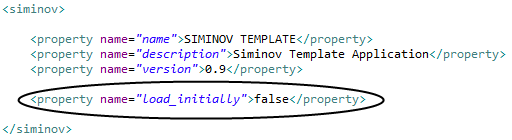
\includegraphics[height=3.5cm]{Resources/siminov_application_template_application_descriptor_load_example.png}
		\end{figure}

		\par
			Basically to map entity and database table, Siminov need DatabaseMappingDescriptor object which defines relation between entity and database table, this object is created by reading DatabaseMappingDescriptor.si.xml file defined by application.

		\par
			\textbf{Lazy Initialization (load\_initially=true)}: If load\_initially is set to true then Siminov will load all descriptors at time of Siminov initialization and will create all its corresponding DatabaseMappingDescriptor objects, and place them in resources layer of Siminov.

		\par
			\textbf{Initial Initialization (load\_initially=false)}: If load\_initially is set to false then Siminov will not load all descriptors at time of Siminov initialization. It will load descriptor only when it is required by Siminov.

\end{enumerate}


\newpage
\section{Handling Multiple Schema's}
Siminov framework supports multiple schema's if required by application. Basically each schema is defined using DatabaseDescriptor.si.xml file. You need to specify all DatabaseDescriptor.si.xml file path in ApplicationDescriptor.si.xml.

		\par
		\textbf{Example:} Siminov Template Application Example.
		\begin{figure}[htbp]
			\centering
				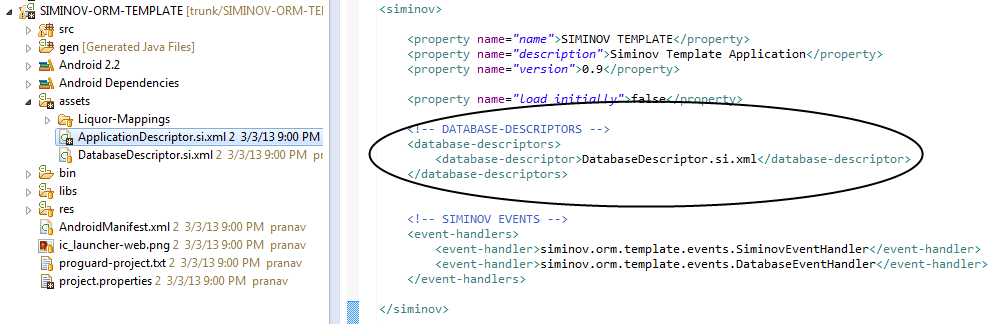
\includegraphics[height=5.5cm]{Resources/siminov_application_multiple_schemas_example.png}
		\end{figure}




%%%%%%%%%%%%%%%%%%%%%%%%%%%%%%%%%%%%%%%%%%%%%%%%%%%%%%%%%%%%%%%%%%%%%%%%%%%%%%%%%%%%%%%%%%%%%%%%%%%%%%%%%%%%%%%%%%%%%%%%
\newpage
\chapter {\Large{Event Notifiers}}

Siminov framework provides few event notifiers which gets triggered based on particular action. Application have to provide implementation for these event notifiers and register them with Siminov.

\section{ISiminov Events} It provide API's related to life cycle of Siminov framework

		\par
		\textbf{Example:} ISiminov Events Notifier
			\lstinputlisting[language=Java]{Resources/isiminov_events_notifier.txt}


		\begin{enumerate}

			\item \small \textbf{First Time Siminov Initialized - firstTimSiminovInitialized()}: It is triggered when Siminov is initialized for first time. In this you can perform tasks which are related to initialization of things only first time of application starts.

					\par
					\textbf{Example:}
	
					\par
					 Preparing initial data for application, which is required by application in its life time, Since it is to be done only once, therefore we will use firstTimeSiminovInitialized API.
					\lstinputlisting[language=Java]{Resources/siminov_template_application_first_time_siminov_initialized_event_notifier_example.txt}	
		
			
					\begin{center}
						\colorbox{grey}{
						\parbox[t]{.8\linewidth}{
							\fontsize{11pt}{11pt}\selectfont % The first argument for fontsize is the font size of the text and the second is the line spacing - you may need to play with these for your particular title
							\vspace*{0.1cm} % Space between the start of the title and the top of the grey box
		
							\hfill \textbf{Note} \\
							This API will be triggered only once when Siminov is initialized first time.
				
							\vspace*{0.0cm} % Space between the end of the title and the bottom of the grey box
						}
					}

					\end{center}


			\item \small \textbf{Siminov Initialized - siminovInitialized()}: It is triggered whenever Siminov is initialized. 

					\begin{center}
						\colorbox{grey}{
						\parbox[t]{.8\linewidth}{
							\fontsize{11pt}{11pt}\selectfont % The first argument for fontsize is the font size of the text and the second is the line spacing - you may need to play with these for your particular title
							\vspace*{0.1cm} % Space between the start of the title and the top of the grey box
		
							\hfill \textbf{Note} \\
								This doesnot gets triggered when Siminov is first time initialized, instead of this firstTimeSiminovInitialized APIwill be triggered.

							\vspace*{0.0cm} % Space between the end of the title and the bottom of the grey box
						}
					}

					\end{center}

		
			\item \small \textbf{Siminov Stopped - siminovStopped()}: It is triggered when Siminov is shutdown.


		\end{enumerate}



\section{IDatabaseEvents} It provide API's related to database operations.


		\par
		\textbf{Example:} IDatabaseEvents Notifier
			\lstinputlisting[language=Java]{Resources/idatabase_events_notifier.txt}


		\begin{enumerate}

			\item \small \textbf{Database Created - databaseCreated(DatabaseDescriptor)}: It is triggered when database is created based on schema defined in DatabaseDescriptor.si.xml file. This API provides DatabaseDescriptor object for which database is created.

			\item \small \textbf{Database Dropped - databaseDropped(DatabaseDescriptor)}: It is triggered when database is dropped. This API provides DatabaseDescriptor object for which database is dropped.


			\item \small \textbf{Table Created - tableCreated(DatabaseMappingDescriptor)}: It is triggered when a table is created in database. This API provides DatabaseMappingDescriptor object which describes table structure.


			\item \small \textbf{Table Dropped - tableDropped(DatabaseMappingDescriptor)}: It is triggered when a table is deleted from database. This API provides DatabaseMappingDescriptor object for which table is dropped.


			\item \small \textbf{Index Created - indexCreated(DatabaseMappingDescriptor, Index)}: It is triggered when a index is created on table. This API provides DatabaseMappingDescriptor and Index object which defines table and index structure.

			
			\item \small \textbf{Index Dropped - indexDropped(DatabaseMappingDescriptor, Index)}: It is triggered when a index is dropped from table. This API provides DatabaseMappingDescriptor and Index object which defines table and index for which index is dropped.

		\end{enumerate}

%%%%%%%%%%%%%%%%%%%%%%%%%%%%%%%%%%%%%%%%%%%%%%%%%%%%%%%%%%%%%%%%%%%%%%%%%%%%%%%%%%%%%%%%%%%%%%%%%%%%%%%%%%%%%%%%%%%%%%%%
\newpage
\chapter {\Large{Database API's}}


\section{Data Types}
Based on java variable type siminov decides the data type of column.

\begin{enumerate}

	\item \small \textbf{int}: Java int primitive data type is converted to \textbf{INTEGER} Sqlite data type.

		\par
		\textbf{Example:} Java int  Primitive Data Type
			\lstinputlisting[language=Java]{Resources/data_type_int_primitive_example.txt}

	\item \small \textbf{Integer}: Java Integer class data type is converted to \textbf{INTEGER} Sqlite data type.

		\par
		\textbf{Example:} Java Integer Class Data Type
			\lstinputlisting[language=Java]{Resources/data_type_integer_class_example.txt}

	\item \small \textbf{long}: Java long primitive data type is converted to \textbf{INTEGER} Sqlite data type.

		\par
		\textbf{Example:} Java long Primitive Data Type
			\lstinputlisting[language=Java]{Resources/data_type_long_primitive_example.txt}

	\item \small \textbf{Long}: Java Long class data type is converted to \textbf{INTEGER} Sqlite data type.

		\par
		\textbf{Example:} Java Long Class Data Type
			\lstinputlisting[language=Java]{Resources/data_type_long_class_example.txt}

	\item \small \textbf{float}: Java float primitive data type is converted to \textbf{REAL} Sqlite data type.

		\par
		\textbf{Example:} Java float Primitive Data Type
			\lstinputlisting[language=Java]{Resources/data_type_float_primitive_example.txt}

	\item \small \textbf{Float}: Java Float class data type is converted to \textbf{REAL} Sqlite data type.

		\par
		\textbf{Example:} Java Float Class Data Type
			\lstinputlisting[language=Java]{Resources/data_type_float_class_example.txt}

	\item \small \textbf{boolean}: Java boolean primitive data type is converted to \textbf{NUMERIC} Sqlite data type.

		\par
		\textbf{Example:} Java boolean Primitive Data Type
			\lstinputlisting[language=Java]{Resources/data_type_boolean_primitive_example.txt}

	\item \small \textbf{Boolean}: Java Boolean class data type is converted to \textbf{NUMERIC} Sqlite data type.

		\par
		\textbf{Example:} Java Boolean Class Data Type
			\lstinputlisting[language=Java]{Resources/data_type_boolean_class_example.txt}

	\item \small \textbf{char}: Java char array primitive data type is converted to \textbf{TEXT} Sqlite data type.

		\par
		\textbf{Example:} Java char Array Primitive Data Type
			\lstinputlisting[language=Java]{Resources/data_type_char_example.txt}

	\item \small \textbf{Character}: Java Character class data type is converted to \textbf{TEXT} Sqlite data type.

		\par
		\textbf{Example:} Java Character Class Data Type
			\lstinputlisting[language=Java]{Resources/data_type_character_class_example.txt}

	\item \small \textbf{String}: Java String class data type is converted to \textbf{TEXT} Sqlite data type.

		\par
		\textbf{Example:} Java String Class Data Type
			\lstinputlisting[language=Java]{Resources/data_type_string_class_example.txt}

	\item \small \textbf{byte}: Java byte array data type is converted to \textbf{NONE} Sqlite data type.

		\par
		\textbf{Example:} Java byte Array Primitive Data Type
			\lstinputlisting[language=Java]{Resources/data_type_byte_primitive_example.txt}

	\item \small \textbf{Byte}: Java Byte class data type is converted to \textbf{NONE} Sqlite data type.

		\par
		\textbf{Example:} Java Byte Class Data Type
			\lstinputlisting[language=Java]{Resources/data_type_byte_class_example.txt}

	\item \small \textbf{void}: Java void primitive data type is converted to \textbf{NONE} Sqlite data type.

		\par
		\textbf{Example:} Java void Primitive Data Type
			\lstinputlisting[language=Java]{Resources/data_type_void_primitive_example.txt}

	\item \small \textbf{Void}: Java Void class data type is converted to \textbf{NONE} Sqlite data type.

		\par
		\textbf{Example:} Java Void Class Data Type
			\lstinputlisting[language=Java]{Resources/data_type_void_class_example.txt}

	\item \small \textbf{short}: Java short primitive is convered to \textbf{INTEGER} Sqlite data type.

		\par
		\textbf{Example:} Java short Primitive Data Type
			\lstinputlisting[language=Java]{Resources/data_type_short_primitive_example.txt}

	\item \small \textbf{Short}: Java Short class data type is converted to \textbf{INTEGER} Sqlite data type.
		
		\par
		\textbf{Example:} Java Short Class Data Type
			\lstinputlisting[language=Java]{Resources/data_type_short_class_example.txt}

\end{enumerate}


\par
Sqlite data types:
	
\begin{enumerate}

	\item \small \textbf{INTEGER Sqlite Data Type}: This sqlite data type generaly contain \textit{INT}, \textit{INTEGER}, \textit{TINYINT}, \textit{SMALLINT}, \textit{MEDIUMINT}, \textit{BIGINT}, \textit{UNSIGNED BIG INT}, \textit{INT2}, \textit{INT8}.
	
	\item \small \textbf{TEXT Sqlite Data Type}: This sqlite data type generaly contain \textit{CHARACTER(20)}, \textit{VARCHAR(255)}, \textit{VARYING CHARACTER(255)}, \textit{NCHAR(55)}, \textit{NATIVE CHARACTER(70)}, \textit{NVARCHAR(100)}, \textit{TEXT}, \textit{CLOB}.

	\item \small \textbf{REAL Sqlite Data Type}: This sqlite data type generaly contain \textit{REAL}, \textit{DOUBLE}, \textit{DOUBLE PRECISION}, \textit{FLOAT}.
	
	\item \small \textbf{NONE Sqlite Data Type}: This sqlite data type generaly contain \textit{BLOB}, \textit{NO DATA TYPE SPECIFIED}.

	\item \small \textbf{NUMERIC Sqlite Data Type}: This sqlite data type generaly contain \textit{NUMERIC}, \textit{DECIMAL(10,5)}, \textit{BOOLEAN}, \textit{DATE}, \textit{DATETIME}.

\end{enumerate}


					\begin{center}
						\colorbox{grey}{
						\parbox[t]{.8\linewidth}{
							\fontsize{11pt}{11pt}\selectfont % The first argument for fontsize is the font size of the text and the second is the line spacing - you may need to play with these for your particular title
							\vspace*{0.1cm} % Space between the start of the title and the top of the grey box
		
							\hfill \textbf{Note} \\
							If you define ORM using Annotation then you dont have to specify data type, it will automatically be configured based on variable data type.
				
							\vspace*{0.0cm} % Space between the end of the title and the bottom of the grey box
						}
					}

					\end{center}



\section{Database API's}
	
	\subsection{Create Database}Siminov provides APIs to create database, based on schema defined in DatabaseDescriptor.si.xml file.

			\textbf{API:} Basically Use IDatabase Interface
				\lstinputlisting[language=Java]{Resources/create_database_api.txt}
		
					\begin{center}
						\colorbox{grey}{
						\parbox[t]{.8\linewidth}{
							\fontsize{11pt}{11pt}\selectfont % The first argument for fontsize is the font size of the text and the second is the line spacing - you may need to play with these for your particular title
							\vspace*{0.1cm} % Space between the start of the title and the top of the grey box
		
							\hfill \textbf{Note} \\
							Generally database creation will be automatically handled by Siminov, but you can do it manually also.

							\textbf{Example:} Manually Creating Database.
								\lstinputlisting[language=Java]{Resources/create_database_api_example.txt}

							\vspace*{0.0cm} % Space between the end of the title and the bottom of the grey box
						}
					}

					\end{center}


	\subsection{Drop Database}Database class provides API to drop complete database of an application.

		\textbf{API}: Drop Database.
		\lstinputlisting[language=Java]{Resources/drop_database_api.txt}
		

		\textbf{Example}
		\lstinputlisting[language=Java]{Resources/drop_database_api_example.txt}



	\subsection{Create Table}Using this API you can create table on database.

			\begin{center}
				\colorbox{grey}{
				\parbox[t]{.8\linewidth}{
					\fontsize{11pt}{11pt}\selectfont % The first argument for fontsize is the font size of the text and the second is the line spacing - you may need to play with these for your particular title
					\vspace*{0.1cm} % Space between the start of the title and the top of the grey box

					\hfill \textbf{Note} \\
					Generally database and its table creation will automatically be handled by Siminov, but u can do it manually also.

					\vspace*{0.0cm} % Space between the end of the title and the bottom of the grey box
					}
			}

			\end{center}


		\par
		There are three ways to create table in database.

		\begin{enumerate}

			\item \small \textbf{Defining table structure using DatabaseMappingDescriptor.si.xml file}

				\textbf{Example}: Liquor.si.xml file Of Siminov Template Application.
				\lstinputlisting[language=XML]{Resources/create_table_example_xml.txt}
		
			\item \small \textbf{Defining table structure using Annotations}

				\textbf{Example}: Liquor Class Of Siminov Template Application.
				\lstinputlisting[language=Java]{Resources/create_table_example_xml_annotation.txt}

			\item \small \textbf{Creating table programmatically}

				\textbf{Example}: Creating Liquor Table Programmatically.
				\lstinputlisting[language=Java]{Resources/create_table_example_programmatically.txt}

		\end{enumerate}


		\par
		 Siminov \textbf{Database} class provide few APIs to create table programmtically.

		\begin{enumerate}

			\item \small \lstinputlisting[language=Java]{Resources/create_table_iterator_of_database_mapping_descriptor_objects.txt}

				\par
				Example:
				\lstinputlisting[language=Java]{Resources/create_table_iterator_of_database_mapping_descriptor_objects_example.txt}

	
			\item \small \lstinputlisting[language=Java]{Resources/create_table_database_mapping_object.txt}

				\par
				Example: Creating Liquor Table Programmatically.
				\lstinputlisting[language=Java]{Resources/create_table_database_mapping_object_example.txt}

		
		\end{enumerate}


	\subsection{Drop Table} Database class provides following API's to drop a table.

		\begin{enumerate}

			\item \small \lstinputlisting[language=Java]{Resources/instance_drop_table_method.txt}

				\par
				\textbf{Example}: Drop Liquor Table Through Liquor Class Object.
				\lstinputlisting[language=Java]{Resources/instance_drop_table_method_example.txt}

			\item \small \lstinputlisting[language=Java]{Resources/static_drop_table_method.txt}

				\par
				\textbf{Example}: Drop Liquor Table Using Static API Of Database.
				\lstinputlisting[language=Java]{Resources/static_drop_table_method_example.txt}

		\end{enumerate}
		

	\subsection{Create Index}
		
		\par
		There are two ways to create index.

		\begin{enumerate}
		
			\item \small \textbf{Define Index Structure Using DatabaseMappingDescriptor.si.xml file}
				\lstinputlisting[language=Java]{Resources/create_index_using_xml.txt}
								
	
			\item \small \textbf{Creating Index Programmatically}
				\par 
				Database class provides few API's two create index programmatically

				\begin{enumerate}

					\item \small \lstinputlisting[language=Java]{Resources/create_index_programmatically_1.txt}

						\par
						\textbf{Example}: 
							\lstinputlisting[language=Java]{Resources/create_index_programmatically_1_example.txt}

					\item \small \lstinputlisting[language=Java]{Resources/create_index_programmatically_2.txt}

						\par
						\textbf{Example}: 
							\lstinputlisting[language=Java]{Resources/create_index_programmatically_2_example.txt}

					\item \small \lstinputlisting[language=Java]{Resources/create_index_programmatically_3.txt}

						\par
						\textbf{Example}:
							\lstinputlisting[language=Java]{Resources/create_index_programmatically_3_example.txt}

					\item \small \lstinputlisting[language=Java]{Resources/create_index_programmatically_4.txt}

						\par
						\textbf{Example}:
							\lstinputlisting[language=Java]{Resources/create_index_programmatically_4_example.txt}

				\end{enumerate}
			

		\end{enumerate}

	\subsection{Drop Index}
		\par 
		Database class provides following API's to drop index from table.
		
		\begin{enumerate}

			\item \small \lstinputlisting[language=Java]{Resources/drop_index_1.txt}

				\par
				\textbf{Example}:
					\lstinputlisting[language=Java]{Resources/drop_index_1_example.txt}

			\item \small \lstinputlisting[language=Java]{Resources/drop_index_2.txt}

				\par
				\textbf{Example}:
					\lstinputlisting[language=Java]{Resources/drop_index_2_example.txt}

		\end{enumerate}
		

	\subsection{Select}

		\par
		Database class provides following API's to fetch tuples from table.

		\begin{enumerate}

			\item \small \lstinputlisting[language=Java]{Resources/select.txt}

				\par
				Fetch tuples from table.

				\textbf{IFetch}: Exposes API's to provide information based on which tuples will be fetched from table.
					\lstinputlisting[language=Java]{Resources/ifetch_interface.txt}
	
			
				\textbf{IFetchClause}: Exposes API's to provide condition to where clause based on which tuples will be fetched from table.
					\lstinputlisting[language=Java]{Resources/ifetchclause_interface.txt}

				\textbf{Example}: Select Liquor Where Type Equal To RUM
					\lstinputlisting[language=Java]{Resources/select_example.txt}

			\item \small \lstinputlisting[language=Java]{Resources/manual_select.txt}

				\par
				Returns all tuples based on manual query from mapped table for invoked class object.

				\textbf{Example}: Select Liquor Object.
					\lstinputlisting[language=Java]{Resources/manual_select_example.txt}


		\end{enumerate}



	\subsection{Save}
		\lstinputlisting[language=Java]{Resources/save.txt}

			\par
			\textbf{Example}: Saving Liquor Object.
				\lstinputlisting[language=Java]{Resources/save_example.txt}


	\subsection{Update}
		\lstinputlisting[language=Java]{Resources/update.txt}

			\par
			\textbf{Example}: Updaing Liquor Object.
				\lstinputlisting[language=Java]{Resources/update_example.txt}


	\subsection{Save Or Update}
		\lstinputlisting[language=Java]{Resources/save_or_update.txt}

			\par
			\textbf{Example}: Save Or Update Liquor Object.
				\lstinputlisting[language=Java]{Resources/save_or_update_example.txt}



			\begin{center}
				\colorbox{grey}{
				\parbox[t]{.8\linewidth}{
					\fontsize{11pt}{11pt}\selectfont % The first argument for fontsize is the font size of the text and the second is the line spacing - you may need to play with these for your particular title
					\vspace*{0.1cm} % Space between the start of the title and the top of the grey box

					\hfill \textbf{Note} \\
					If tuple is not present in table then it will insert it into table else it will update the tuple.

					\vspace*{0.0cm} % Space between the end of the title and the bottom of the grey box
					}
			}

			\end{center}


	\subsection{Delete}
		\par 
		Database class provides following API's to delete tuples from table.

			\textbf{API}: Delete API.
				\lstinputlisting[language=Java]{Resources/delete.txt}
		
			\textbf{IDelete}:  Exposes API's to delete tuples from table.

				\lstinputlisting[language=Java]{Resources/idelete.txt}

			
			\textbf{IDeleteClause}: Exposes API's to provide condition on where clause to delete tuple from table.
				\lstinputlisting[language=Java]{Resources/ideleteclause.txt}

			\textbf{Example}: 
				\lstinputlisting[language=Java]{Resources/delete_example.txt}
	

\section{Database Siminov API's}


	\subsection{Get Database Descriptor}
	\lstinputlisting[language=Java]{Resources/get_database_descriptor.txt}

				\par
				\textbf{Example}: Get Database Descriptor Object Which Contain Liquor Table.
					\lstinputlisting[language=Java]{Resources/get_database_descriptor_example.txt}


	\subsection{Get Database Mapping Descriptor}
	\lstinputlisting[language=Java]{Resources/get_database_mapping.txt}

				\par
				\textbf{Example}: Get Database Mapping Descriptor Object Related To Liquor Table.
					\lstinputlisting[language=Java]{Resources/get_database_mapping_example.txt}


	\subsection{Get Table Name}
	\lstinputlisting[language=Java]{Resources/get_table_name.txt}

				\par
				\textbf{Example}: Get Liquor Object Table Name.
					\lstinputlisting[language=Java]{Resources/get_table_name_example.txt}
		

	\subsection{Get Column Names}
	\lstinputlisting[language=Java]{Resources/get_column_names.txt}

				\par
				\textbf{Example}: Get All Column Names Of Liquor Table.
					\lstinputlisting[language=Java]{Resources/get_column_names_example.txt}


	\subsection{Get Column Values}
	\lstinputlisting[language=Java]{Resources/get_column_values.txt}

				\par
				\textbf{Example}: Get All Column Values Of Liquor Object.
					\lstinputlisting[language=Java]{Resources/get_column_values_example.txt}


	\subsection{Get Column Types}
	\lstinputlisting[language=Java]{Resources/get_column_types.txt}

				\par
				\textbf{Example}: Get All Column Types Of Liquor Table.
					\lstinputlisting[language=Java]{Resources/get_column_types_example.txt}


	\subsection{Get Primary Keys}
	\lstinputlisting[language=Java]{Resources/get_primary_keys.txt}

				\par
				\textbf{Example}: Get All Primary Keys Of Liquor Table.
					\lstinputlisting[language=Java]{Resources/get_primary_keys_example.txt}


	\subsection{Get Mandatory Fields}
	\lstinputlisting[language=Java]{Resources/get_mandatory_fields.txt}

				\par
				\textbf{Example}: Get All Column Names Which Are Marked As Manadatory Fields.
					\lstinputlisting[language=Java]{Resources/get_mandatory_fields_example.txt}

	\subsection{Get Unique Fields}
	\lstinputlisting[language=Java]{Resources/get_unique_fields.txt}

				\par
				\textbf{Example}: Get All Column Names Which Are Marked As Unique.
					\lstinputlisting[language=Java]{Resources/get_unique_fields_example.txt}


	\subsection{Get Foreign Keys}
	\lstinputlisting[language=Java]{Resources/get_foreign_keys.txt}

				\par
				\textbf{Example}: Get All Column Names Which Are Marked As Foreign Keys.
					\lstinputlisting[language=Java]{Resources/get_foreign_keys_example.txt}


\section{Database Aggregation API's}


	\subsection{Count}
		\par
		Returns the count of rows based on information provided.

			\textbf{API}: Count API.
				\lstinputlisting[language=Java]{Resources/count.txt}
		
			\textbf{ICount}:  Exposes API's to get count of the number of times that X is not NULL in a group.
						 The count(*) function (with no arguments) returns the total number of rows in the group.

				\lstinputlisting[language=Java]{Resources/icount_interface.txt}

			
			\textbf{ICountClause}: Exposes API's to provide condition on where clause to calculate count.
				\lstinputlisting[language=Java]{Resources/icountclause_interface.txt}

			\textbf{Example}: Get count of liquors type equal to RUM.
				\lstinputlisting[language=Java]{Resources/count_example.txt}


	\subsection{Average} 
		\par 
		Returns the average based on column name provided.

			\textbf{API}: Average API.
				\lstinputlisting[language=Java]{Resources/average.txt}
		
			\textbf{IAverage}:  Exposes API's to get average value of all non-NULL X within a group. 
 						 String and BLOB values that do not look like numbers are interpreted as 0.
						 The result of avg() is always a floating point value as long as at there is at least one non-NULL input even if all inputs are integers.
						 The result of avg() is NULL if and only if there are no non-NULL inputs.

				\lstinputlisting[language=Java]{Resources/iaverage_interface.txt}

			
			\textbf{IAverageClause}: Exposes API's to provide condition on where clause to calculate average.
				\lstinputlisting[language=Java]{Resources/iaverageclause_interface.txt}

			\textbf{Example}: 
				\lstinputlisting[language=Java]{Resources/average_example.txt}
		

	\subsection{Sum} 
		\par 
		Returns the sum based on column name provided.

			\textbf{API}: Sum API.
				\lstinputlisting[language=Java]{Resources/sum.txt}
		
			\textbf{ISum}:   Exposes API's to return sum of all non-NULL values in the group.
					  	 If there are no non-NULL input rows then sum() returns NULL but total() returns 0.0.
						 NULL is not normally a helpful result for the sum of no rows but the SQL standard requires it and most other SQL database engines implement sum() that way so SQLite does it in the same way in order to be compatible.
						 The result of sum() is an integer value if all non-NULL inputs are integers. 

				\lstinputlisting[language=Java]{Resources/isum_interface.txt}

			
			\textbf{ISumClause}: Exposes API's to provide condition on where clause to calculate sum.
				\lstinputlisting[language=Java]{Resources/isumclause_interface.txt}

			\textbf{Example}: 
				\lstinputlisting[language=Java]{Resources/sum_example.txt}


	\subsection{Total} 
		\par 
		Returns the total based on column name provided.

			\textbf{API}: Total API.
				\lstinputlisting[language=Java]{Resources/total.txt}
		
			\textbf{ITotal}:     Exposes API's to return total of all non-NULL values in the group.
 						The non-standard total() function is provided as a convenient way to work around this design problem in the SQL language.
						The result of total() is always a floating point value.


				\lstinputlisting[language=Java]{Resources/itotal_interface.txt}

			
			\textbf{ITotalClause}: Exposes API's to provide condition on where clause to calculate total.
				\lstinputlisting[language=Java]{Resources/itotalclause_interface.txt}

			\textbf{Example}: 
				\lstinputlisting[language=Java]{Resources/total_example.txt}


	\subsection{Minimum} 
		\par 
		Returns the minimum based on column name provided.

			\textbf{API}: Minimum API.
				\lstinputlisting[language=Java]{Resources/minimum.txt}
		
			\textbf{IMin}:      Exposes API's to returns the minimum non-NULL value of all values in the group.
						The minimum value is the first non-NULL value that would appear in an ORDER BY of the column.
						Aggregate min() returns NULL if and only if there are no non-NULL values in the group.


				\lstinputlisting[language=Java]{Resources/iminimum_interface.txt}

			
			\textbf{IMinClause}: Exposes API's to provide condition on where clause to calculate minimum.
				\lstinputlisting[language=Java]{Resources/iminimumclause_interface.txt}

			\textbf{Example}: 
				\lstinputlisting[language=Java]{Resources/minimum_example.txt}



	\subsection{Maximum} 
		\par 
		Returns the minimum based on column name provided.

			\textbf{API}: Maximum API.
				\lstinputlisting[language=Java]{Resources/maximum.txt}
		
			\textbf{IMax}:    Exposes API's to returns the maximum value of all values in the group.
						The maximum value is the value that would be returned last in an ORDER BY on the same column. 
						Aggregate max() returns NULL if and only if there are no non-NULL values in the group.


				\lstinputlisting[language=Java]{Resources/imax_interface.txt}

			
			\textbf{IMaxClause}: Exposes API's to provide condition on where clause to calculate maximum.
				\lstinputlisting[language=Java]{Resources/imaxclause_interface.txt}

			\textbf{Example}: 
				\lstinputlisting[language=Java]{Resources/maximum_example.txt}


	\subsection{Group Concat} 
		\par 
		Returns the group concat based on column name provided.

			\textbf{API}: Group Concat API.
				\lstinputlisting[language=Java]{Resources/groupconcat.txt}
		
			\textbf{IGroupConcat}:     Exposes API's to get group concat that returns a string which is the concatenation of all non-NULL values of X.
							If parameter Y is present then it is used as the separator between instances of X. A comma (",") is used as the separator if Y is omitted.
							The order of the concatenated elements is arbitrary.


				\lstinputlisting[language=Java]{Resources/igroupconcat_interface.txt}

			
			\textbf{IGroupConcatClause}: Exposes API's to provide condition on where clause to calculate group concat.
				\lstinputlisting[language=Java]{Resources/igroupconcatclause_interface.txt}

			\textbf{Example}: 
				\lstinputlisting[language=Java]{Resources/groupconcat_example.txt}


\section{Database Transaction API's}

	\subsection{Begin Transaction}
	\lstinputlisting[language=Java]{Resources/begin_transaction.txt}

	\par
	Begins a transaction in \textbf{EXCLUSIVE} mode.

	\par
	Transactions can be nested. When the outer transaction is ended all of the work done in that transaction and all of the nested transactions will be committed or rolled back. The changes will be rolled back if any transaction is ended without being marked as clean(by calling commitTransaction). Otherwise they will be committed.

				\par
				\textbf{Example}: Saving Liquor Within Transaction.
					\lstinputlisting[language=Java]{Resources/begin_transaction_example.txt}


	\subsection{Commit Transaction}
	\lstinputlisting[language=Java]{Resources/commit_transaction.txt}

	\par
	Marks the current transaction as successful. Finally it will End a transaction.

				\par
				\textbf{Example}: Save And Commt Liquor Transaction.
					\lstinputlisting[language=Java]{Resources/commit_transaction_example.txt}

	
	\subsection{End Transaction}
	\lstinputlisting[language=Java]{Resources/end_transaction.txt}

	\par
	End the current transaction.

				\par
				\textbf{Example}: End Transaction After Save And Commit Transaction.
					\lstinputlisting[language=Java]{Resources/end_transaction_example.txt}


\section{Making Transaction Thread Safe}
By default any transaction executed on database is not thread safe, android provides API to make all transaction thread-safe by using locks around critical sections. This is pretty expensive, so if you know that your DB will nly be used by a single thread then you should not use this in your application.

	\par
	\textbf{Android API}: setLockingEnabled Enable/Disable
		\lstinputlisting[language=Java]{Resources/andorid_transaction_set_locking_enabled_api.txt}

Configuring transaction thread-safe in Siminov. To enable/disable transaction thread-safe in Siminov you have to use property is\_locking\_required defined in DatabaseDescriptor.si.xml file.

		\par
		\textbf{Example:} Siminov Template Application DatabaseDescriptor.si.xml file.
		\begin{figure}[htbp]
			\centering
				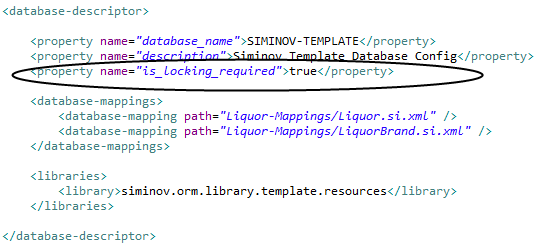
\includegraphics[height=7cm]{Resources/siminov_template_application_is_locking_enable_example.png}
		\end{figure}


\section{Preparing Where Clause}
Siminov does not provide any mechanism to prepare where-clause, Providing where-clause for fetch API is easy. It take same syntax as we form where-clause for SQLite statement.

\textbf{Example}: Fetch Liquor tuple where liquor type is Beer.
	\lstinputlisting[language=Java]{Resources/preparing_where_clause.txt}
	


\section{Handling Database Relationships}

	\subsection{One to One}
	One-To-One relationship is in which each row in one database table is linked to 1 and 1 other row in another table.

	\textbf{Example}: Relationship between Table A and Table B, each row in Table A is linked to another row in Table B. The number of rows in Table A must equal the number of rows in Table B.

	\textbf{One To One Syntax}: 
		\lstinputlisting[language=Java]{Resources/one_to_one_syntax.txt}

	\subsection{One to Many}
	One-To-Many relationship is in which each row in the related to table can be related to many rows in the relating table. This effectively save storage as the related record does not need to be stored multiple times in the relating table.

	\textbf{Example}: All the customers belonging to a business is stored in a customer table while all the customer invoices are stored in an invoice table. Each customer can have many invoices but each invoice can only be generated for a single customer.	
			
	\textbf{One To Many Syntax}: 
		\lstinputlisting[language=Java]{Resources/one_to_many_syntax.txt}

	\subsection{Many to One}
	Many-To-One relationship is in which one entity (typically a column or set of columns) contains values that refer to another entity (a column or set of columns) that has unique values.

	\textbf{Example}: In a geography schema having tables Region, State, and City, there are many states that are in a given region, but no states are in two regions.
	
	\textbf{Many To One Syntax}: 
		\lstinputlisting[language=Java]{Resources/many_to_one_syntax.txt}

	\subsection{Many to Many}
	Many-To-Many relationship is in which one or more rows in the table can be related to 0, 1 or many rows in another table. A mapping table is required in order to implement  such a relationship.

	\textbf{Example}: All the customers belonging to a bank is stored in a customer table while all the bank's products are stored in a product table. Each customer can have many products and each product can be assigned to many customers.
	
	\textbf{Many To Many Syntax}: 
		\lstinputlisting[language=Java]{Resources/many_to_many_syntax.txt}



%%%%%%%%%%%%%%%%%%%%%%%%%%%%%%%%%%%%%%%%%%%%%%%%%%%%%%%%%%%%%%%%%%%%%%%%%%%%%%%%%%%%%%%%%%%%%%%%%%%%%%%%%%%%%%%%%%%%%%%%
\newpage
\chapter {\Large{Database Upgrade}}
Over time the requirement of the database within the application may change, this is almost inevitable if your application is in active development and you're constantly adding new features. Properly upgrading the database in application is important, because if something goes wrong application will have unexpected behaviour (such as crashing) or app may may loose its all data and have to start over.

\textbf{SQLite Limitation}: SQLite supports a limited subset of ALTER TABLE. The ALTER TABLE command in SQLite allows the user to rename a tablet or to add a new column to an existing table. It is not possible to rename a column, remove a column, or add or remove constraints from a table. But you can alter table column datatype or other property by the following steps:

\begin{enumerate}

	\item \small BEGIN TRANSACTION
	\item \small CREATE TEMPORARY TABLE t1\_backup(a, b);
	\item \small INSERT INTO t1\_backup SELECT a, b FROM t1;
	\item \small DROP TABLE
	\item \small CREATE TABLE t1(a, b);
	\item \small INSERT INTO t1 SELECT a, b FROM t1\_backup;
	\item \small DROP TABLE t1\_backup;
	\item \small COMMIT

\end{enumerate}

For more detail you can refer the \url{http://www.sqlite.org/lang_altertable.html}

\section{Siminov Database Upgrade}Siminov provides easy way to upgrade application database. It only support adding new table to existing database, adding a new column to existing table, and deleting existing table.

		\par
		\textbf{Example:} Siminov Template Application DatabaseDescriptor.si.xml file.
		\begin{figure}[htbp]
			\centering
				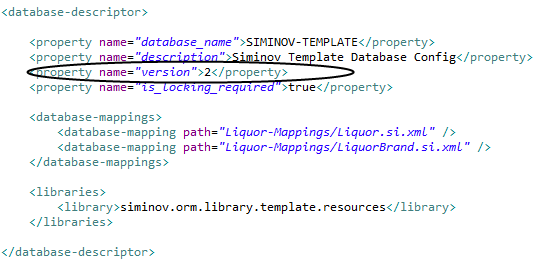
\includegraphics[height=7cm]{Resources/siminov_template_application_database_version.png}
		\end{figure}

\begin{center}
	\colorbox{grey}{
		\parbox[t]{.8\linewidth}{
			\fontsize{11pt}{11pt}\selectfont % The first argument for fontsize is the font size of the text and the second is the line spacing - you may need to play with these for your particular title
			\vspace*{0.1cm} % Space between the start of the title and the top of the grey box
		
			\hfill \textbf{Note} \\

			\hfill 	
			\begin{enumerate}
			
				\item \small Database Version should not contain decimal value.

			\end{enumerate}

			\vspace*{0.0cm} % Space between the end of the title and the bottom of the grey box
		}
	}

\end{center}

%%%%%%%%%%%%%%%%%%%%%%%%%%%%%%%%%%%%%%%%%%%%%%%%%%%%%%%%%%%%%%%%%%%%%%%%%%%%%%%%%%%%%%%%%%%%%%%%%%%%%%%%%%%%%%%%%%%%%%%%
\newpage
\chapter {\Large{Database Encryption}}
Data Secuirty plays important role when we talk about database. It protect your database from desctructive forces and the unwanted actions of unauthorized users.

\par
Android sqlite does not provide any protection against your database. There are many third party security implementation's which application developer can use in their application to protect their database.

\section{SQLCipher}
SQLCipher is an open source extension to SQLite that provides transparent 256-bit AES encryption of database file. SQLCipher has a small footprint and great performance so it's ideal for protecting embedded application databases and is well suited for mobile development.

\par
Siminov provide implementation for SQLCipher database encryption security. Its easy and secured to use it.

\par
Below are steps to make your application totally secured.

\begin{enumerate}

	\item \small Download SQLCipher from their website for android (\url{http://sqlcipher.net/downloads/}).

	\item \small Configure SQLCipher in your application. Follow below steps:

		\begin{enumerate}

			\newpage
			\item \small Copy \textbf{sqlcipher.jar}, \textbf{guava-r09.jar}, \textbf{commons-codec.jar} in your application libs folder.

				\begin{figure}[!htbp]
					\centering
						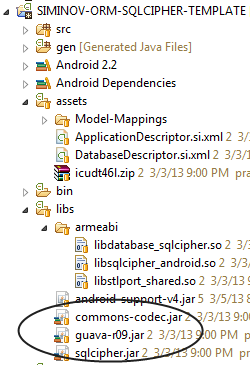
\includegraphics[height=8cm]{Resources/siminov_template_sqlcipher_application_setup_1.png}
					\end{figure}

			\item \small Copy dll file in your libs folder. 

				\begin{figure}[!htbp]
					\centering
						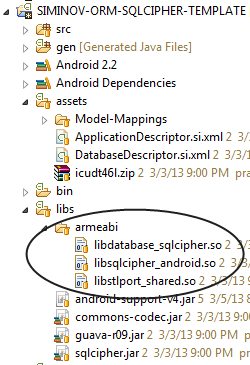
\includegraphics[height=8cm]{Resources/siminov_template_sqlcipher_application_setup_2.png}
					\end{figure}

		
			\newpage		
			\item \small Copy icudt461.zip in your application assets folder.

				\begin{figure}[!htbp]
					\centering
						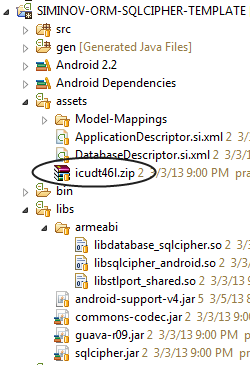
\includegraphics[height=8cm]{Resources/siminov_template_sqlcipher_application_setup_3.png}
					\end{figure}

		\end{enumerate}

		\par
		The stucture of your application should look like this.
	
				\begin{figure}[!htbp]
					\centering
						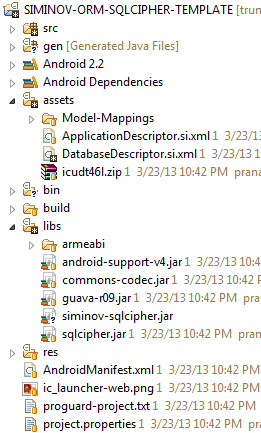
\includegraphics[height=8cm]{Resources/siminov_template_sqlcipher_application_setup.png}
					\end{figure}
	
	\newpage
	\item \small Download and copy Siminov SQLCipher jar in application libs folder.

				\begin{figure}[!htbp]
					\centering
						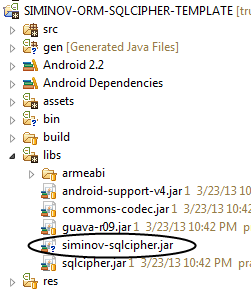
\includegraphics[height=7cm]{Resources/siminov_sqlcipher_template_application_add_siminov_sqlcipher_jar.png}
					\end{figure}

	\item \small To configure SQLCipher with Siminov add type property as sqlcipher and password attribute in DatabaseDescriptor.si.xml.

				\begin{figure}[!htbp]
					\centering
						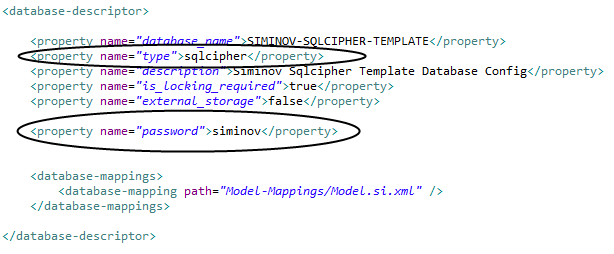
\includegraphics[height=4.3cm]{Resources/siminov_template_sqlcipher_application_sqlcipherdatabaseimpl_class_configure.png}
					\end{figure}

\end{enumerate}


					\begin{center}
						\colorbox{grey}{
						\parbox[t]{.8\linewidth}{
							\fontsize{11pt}{11pt}\selectfont % The first argument for fontsize is the font size of the text and the second is the line spacing - you may need to play with these for your particular title
							\vspace*{0.1cm} % Space between the start of the title and the top of the grey box
		
							\hfill \textbf{Note} \\
							For any future reference you can download SIMINOV-SQLCIPHER-TEMPLATE Application and can check how we have configured application with SQLCipher.
			

							\vspace*{0.0cm} % Space between the end of the title and the bottom of the grey box
						}
					}

					\end{center}

%%%%%%%%%%%%%%%%%%%%%%%%%%%%%%%%%%%%%%%%%%%%%%%%%%%%%%%%%%%%%%%%%%%%%%%%%%%%%%%%%%%%%%%%%%%%%%%%%%%%%%%%%%%%%%%%%%%%%%%%
\newpage
\chapter {\Large{Database Layer}}

Database is the most important part of Siminov ORM. It provides an easy way to implement your own database layer, all you have to do is provide implementation for below interface's. 

\section{IDatabase Interface}
Exposes methods to deal with actual database object. It has methods to open, create, close, and execute query's. 

\lstinputlisting[language=Java]{Resources/idatabase_interface.txt}


\begin{enumerate}

	\item \small \textbf{Open Or Create - openOrCreate(Path)}: Open/Create the database through Database Descriptor. By default add CREATE\_IF\_NECESSARY flag so that if database does not exist it will create.

		\textbf{Example}: 
			\lstinputlisting[language=Java]{Resources/idatabase_open_or_create_api_example.txt}


	\item \small \textbf{Close - close()}: Close the existing opened database through Database Descriptor.

		\textbf{Example}: 
			\lstinputlisting[language=Java]{Resources/idatabase_close_api_example.txt}

	\item \small \textbf{Execute Query - executeQuery(Query)}: Execute a single SQL statement that is NOT a SELECT or any other SQL statement that returns data. It has no means to return any data (such as the number of affected rows). Instead, you're encouraged to use insert, update, delete, when possible. 
	
		\textbf{Example}: 
			\lstinputlisting[language=Java]{Resources/idatabase_execute_query_api_example.txt}

	\item \small \textbf{Execute Bind Query - executeBindQuery(Query, Column Values)}: A pre-compiled statement that can be reused. The statement cannot return multiple rows, but 1x1 result sets are allowed.
 
		\textbf{Example}: 
			\lstinputlisting[language=Java]{Resources/idatabase_execute_bind_query_api_example.txt}

	\item \small \textbf{Execute Fetch Query - executeFetchQuery(Query)}: Query the given table, returning a Cursor over the result set.

		\textbf{Example}: 
			\lstinputlisting[language=Java]{Resources/idatabase_execute_fetch_query_api_example.txt}

	\item \small \textbf{Execute Method - executeMethod(Method Name, Parameters)}: Executes the method on database object.

		\textbf{Example}: 
			\lstinputlisting[language=Java]{Resources/idatabase_execute_method_api_example.txt}

\end{enumerate}


\section{IDataTypeHandler}
Exposes convert API which is responsible to provide column data type based on java variable data type.

\lstinputlisting[language=Java]{Resources/idatatypehandler_interface.txt}


\begin{enumerate}
	
	\item \small \textbf{Convert Data Type - convert()}: Converts java variable data type to database column data type.

\end{enumerate}


\section{IQueryBuilder}
Exposes API's to build database queries.

\lstinputlisting[language=Java]{Resources/iquerybuilder_interface.txt}



%%%%%%%%%%%%%%%%%%%%%%%%%%%%%%%%%%%%%%%%%%%%%%%%%%%%%%%%%%%%%%%%%%%%%%%%%%%%%%%%%%%%%%%%%%%%%%%%%%%%%%%%%%%%%%%%%%%%%%%%
\newpage
\chapter {\Large{Handling Libraries}}

An Android library project is a development project that holds shared Android source code and resources. Other Andriod application projects can reference the library project and, at build time, include its compiled sources in their .apk files. Multiple application projects can reference the same library project and any single application project can reference multiple library projects.

\par
Siminov provides mechnism to configure ORM for your library projects. 


\section{Setting up a Library Project}

\begin{enumerate}

	\item \small In the \textbf{Package Explorer}, right-click the library project and select \textbf{Properties}.

	\item \small In the \textbf{Properties} window, select the Andorid properties group at left and locate the \textbf{Library} properties at right.

	\item \small Select the is Library checkbox and click \textbf{Apply}.

	\item \small Click \textbf{OK} to close the properties window.

\end{enumerate}

		\begin{figure}[!htbp]
			\centering
				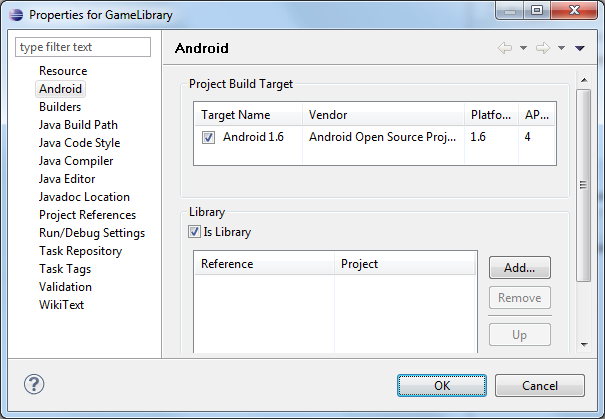
\includegraphics[height=10cm]{Resources/setting_up_a_library_project.png}
		\end{figure}

\newpage
\section{Referencing a library project}
\begin{enumerate}

	\item \small In the \textbf{Package Explorer}, right-click the depedent project and select \textbf{Properties}.

	\item \small In the \textbf{Properties} window, select the Android properties group at left and locate the \textbf{Library} properties at right.
	
	\item \small Click \textbf{Add} to open the \textbf{Project Selection} dialog.

	\item \small From the list of available library project, select a project and click \textbf{OK}.

	\item \small When the dialog closes, click \textbf{Apply} in the \textbf{Properties} window.

	\item \small Click \textbf{OK} to close the \textbf{Properties} window.
	
\end{enumerate}

\newpage
		\begin{figure}[!htbp]
			\centering
				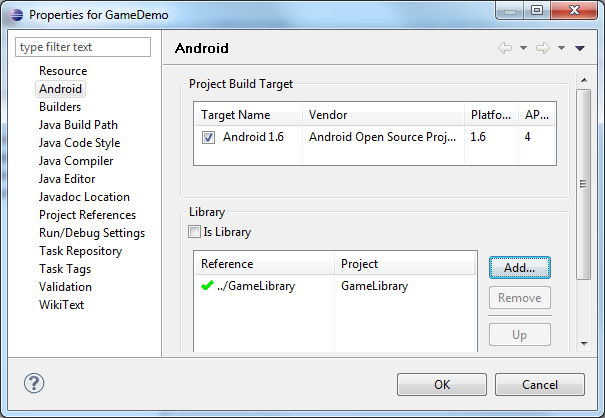
\includegraphics[height=10cm]{Resources/referencing_a_library_project.png}
		\end{figure}

\newpage
\section{Configure Application With Library}

\begin{enumerate}

	\item \small Define LibraryDescriptor.si.xml file for your library project.
	
		\begin{figure}[!htbp]
			\centering
				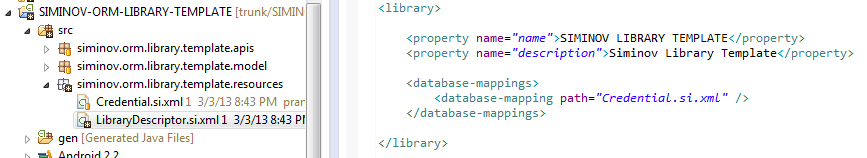
\includegraphics[height=3.5cm]{Resources/siminov_library_template_library_descriptor.png}
		\end{figure}

		\begin{center}
			\colorbox{grey}{
			\parbox[t]{.8\linewidth}{
				\fontsize{11pt}{11pt}\selectfont % The first argument for fontsize is the font size of the text and the second is the line spacing - you may need to play with these for your particular title
				\vspace*{0.1cm} % Space between the start of the title and the top of the grey box
		
				\hfill \textbf{Note} \\
					LibraryDescriptor.si.xml file should not be place in assets folder. Create new package and place all descriptors in that.

				\vspace*{0.0cm} % Space between the end of the title and the bottom of the grey box
				}
			}

		\end{center}


	\item \small Configure LibraryDescriptor.si.xml in your application.
			
		\begin{figure}[!htbp]
			\centering
				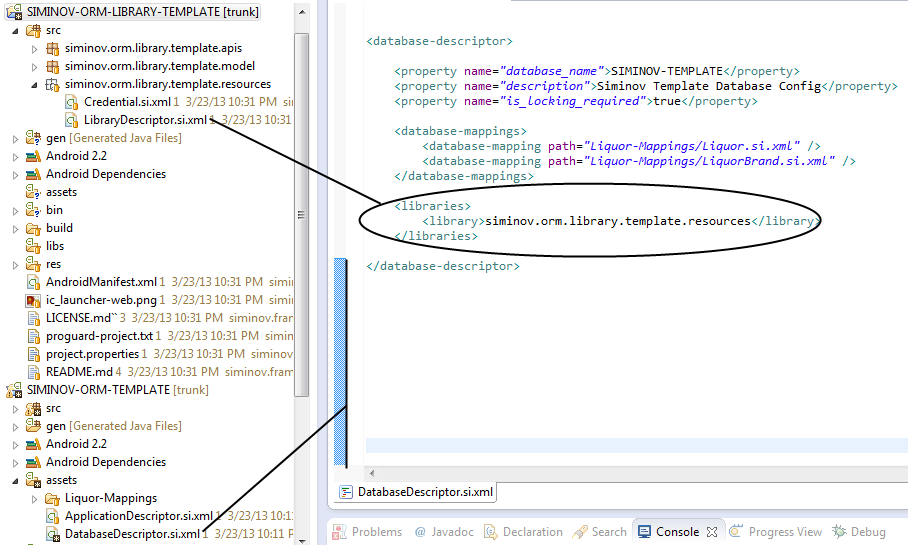
\includegraphics[height=10cm]{Resources/siminov_library_template_configure.png}
		\end{figure}

		\begin{center}
			\colorbox{grey}{
			\parbox[t]{.8\linewidth}{
				\fontsize{11pt}{11pt}\selectfont % The first argument for fontsize is the font size of the text and the second is the line spacing - you may need to play with these for your particular title
				\vspace*{0.1cm} % Space between the start of the title and the top of the grey box
		
				\hfill \textbf{Note} \\
					While configuring DatabaseDescriptor.si.xml file you need to provide full library package name in which LibraryDescriptor.si.xml file is defined.

				\vspace*{0.0cm} % Space between the end of the title and the bottom of the grey box
				}
			}

		\end{center}



\end{enumerate}

%%%%%%%%%%%%%%%%%%%%%%%%%%%%%%%%%%%%%%%%%%%%%%%%%%%%%%%%%%%%%%%%%%%%%%%%%%%%%%%%%%%%%%%%%%%%%%%%%%%%%%%%%%%%%%%%%%%%%%%%
\newpage
\chapter {\Large{Siminov ORM Architecture}}

\begin{figure}[!htbp]
	\centering
		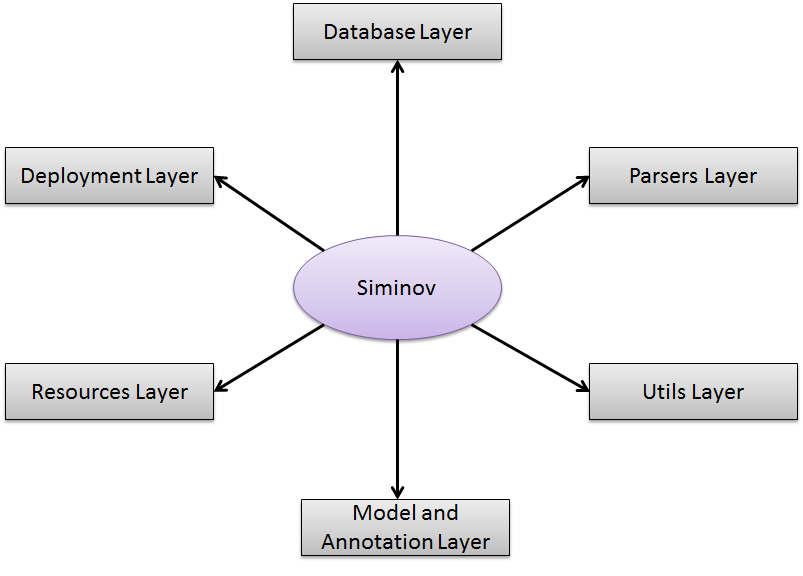
\includegraphics[height=8cm]{Resources/siminov_layers.png}
	\caption{Siminov ORM Layers}
\end{figure}


\newpage
\section{Deployment Layer}
When application starts for first time it does not have its database's. Siminov provides deployment layer, it creates application database's by reading all descriptors from application assests and its libraries.

\textbf{\subsection{siminov.orm.Siminov}}

		\lstinputlisting[language=Java]{Resources/siminov_class.txt}


\newpage
\section{Resources Layer}
It holds meta data about application needed by Siminov. 

\textbf{\subsection{siminov.orm.Resources}} Only GET APIS shown, for rest visit Javadoc
		\lstinputlisting[language=Java]{Resources/resources_class.txt}


\newpage
\section{Database Layer}
This layer basically deals with database operations.

\textbf{\subsection{siminov.orm.database.Database}}
	
		\lstinputlisting[language=Java]{Resources/database_class.txt}


\newpage
\section{Model and Annotation Layer}
It holds Model POJO classes and Annotation defination required for database mapping descriptor.


\textbf{\subsection{siminov.orm.model.ApplicationDescriptor}}

	
		\lstinputlisting[language=Java]{Resources/application_descriptor_class.txt}
		
\newpage
\textbf{\subsection{siminov.orm.model.DatabaseDescriptor}}

		\lstinputlisting[language=Java]{Resources/database_descriptor_class.txt}

	
\newpage
\textbf{\subsection{siminov.orm.model.LibraryDescriptor}}

		\lstinputlisting[language=Java]{Resources/library_descriptor_class.txt}


\newpage
\textbf{\subsection{siminov.orm.model.DatabaseMappingDescriptor}}

		\lstinputlisting[language=Java]{Resources/database_mapping_descriptor_class.txt}


\newpage
\textbf{\subsection{siminov.orm.annotation.Table}}

		\lstinputlisting[language=Java]{Resources/table_annotation_interface.txt}

	
\newpage
\textbf{\subsection{siminov.orm.annotation.Column}}

		\lstinputlisting[language=Java]{Resources/column_annotation_interface.txt}

	
\newpage
\textbf{\subsection{siminov.orm.annotation.Property}}

		\lstinputlisting[language=Java]{Resources/properties_annotation_interface.txt}

\newpage
\textbf{\subsection{siminov.orm.annotation.Index}}

		\lstinputlisting[language=Java]{Resources/index_annotation_interface.txt}

\newpage
\textbf{\subsection{siminov.orm.annotation.IndexColumn}}

		\lstinputlisting[language=Java]{Resources/index_column_annotation_interface.txt}

	
\newpage
\textbf{\subsection{siminov.orm.annotation.Indexes}}

		\lstinputlisting[language=Java]{Resources/indexes_annotation_interface.txt}


\newpage
\textbf{\subsection{siminov.orm.annotation.Reference}}

		\lstinputlisting[language=Java]{Resources/reference_annotation_interface.txt}


\newpage
\textbf{\subsection{siminov.orm.annotation.Map}}

		\lstinputlisting[language=Java]{Resources/map_annotation_interface.txt}


\newpage
\section{Parsers Layer}
It contain parses which parses all descriptor defined by application.


\textbf{\subsection{siminov.orm.parsers.ApplicationDescriptorParser}}
It is used to parse ApplicationDescriptor.si.xml files defined by application.
	
\textbf{\subsection{siminov.orm.parsers.DatabaseDescriptorParser}}
It is used to parse DatabaseDescriptor.si.xml files defined by application.
	
\textbf{\subsection{siminov.orm.parsers.LibraryDescriptorParser}}
It is used to parse LibraryDescriptor.si.xml files defined by application.
	
\textbf{\subsection{siminov.orm.parsers.DatabaseMappingDescriptor}}
It is used to parse DatabaseMappingDescriptor.si.xml files defined by application.


\newpage
\section{Utils Layer}
It provides util classes which provides additional befinites.

\textbf{\subsection{siminov.orm.utils.Utils}}

		\lstinputlisting[language=Java]{Resources/utils_class.txt}


%%%%%%%%%%%%%%%%%%%%%%%%%%%%%%%%%%%%%%%%%%%%%%%%%%%%%%%%%%%%%%%%%%%%%%%%%%%%%%%%%%%%%%%%%%%%%%%%%%%%%%%%%%%%%%%%%%%%%%%%
\newpage
\chapter {\Large{Exceptions}}

\section{Siminov Exception}
	\lstinputlisting[language=Java]{Resources/siminov_exception_class.txt}

\par
This is general exception, which is thrown through Siminov API, if any exception occur while performing any tasks.

\section{Deployment Exception}
	\lstinputlisting[language=Java]{Resources/deployment_exception_class.txt}

\par
This is runtime-time exception, which is thrown if any exception occur at time of initialization of Siminov.

\section{Database Exception}
	\lstinputlisting[language=Java]{Resources/database_exception_class.txt}

\par
This is general exception, which is thrown through Siminov database API's, if any exception occur which doing any database operations.

\end{document}